% Making some of the graphics:
% tgif -print -color -eps wvs-146-1.obj; epstopdf wvs-146-1.eps
% tgif -print -color -eps wvs-146-2.obj; epstopdf wvs-146-2.eps
% tgif -print -color -eps wvs-146-3.obj; epstopdf wvs-146-3.eps
% Other graphics were made by maple; .eps and .pdf are checked in

\documentclass[11pt]{article}
\usepackage{alltt}
\usepackage[fleqn]{empheq} % 
\usepackage{amsmath}
\usepackage{floatflt}
\usepackage{graphicx}
\usepackage{longtable}
\usepackage[strings]{underscore}

\textwidth 6.5in
\oddsidemargin -0.25in
%\evensidemargin -0.5in
\topmargin -0.5in
\textheight 9in

\newcommand{\docname}{wvs-146r10}
\newcommand{\docdate}{7 April 2020}

\ifx\pdfoutput\undefined
  \pdfoutput=0
\fi
\ifnum\pdfoutput>0

  \usepackage[pdftex,plainpages,hyperindex=true,pdfpagelabels]{hyperref}
  \hypersetup{%
    hypertexnames=false,%
    colorlinks=true,%
    linktocpage=true,%
  }
  % Specify the driver for the color package
  \ExecuteOptions{pdftex}
\else
  \usepackage[hypertex,plainpages,hyperindex=true]{hyperref}
  \hypersetup{%
    hypertexnames=false%
  }
  % Specify the driver for the color package
  \ExecuteOptions{dvips}
  %\ExecuteOptions{xdvi}
\fi

\hyperbaseurl{}
\newcommand\hr[1]{\href{#1.dvi}{dvi}, \href{#1.pdf}{pdf}}
\newcommand\h[1]{#1 (\hr{#1})}

\newcommand{\degs}{$\stackrel{\hspace*{-0.5pt}^\circ}{\vspace*{-2pt}.}$}
\newcommand{\mdegs}{\stackrel{\hspace*{-0.5pt}^\circ}{\vspace*{-2pt}.}}

\begin{document}

%\tracingcommands=1
\newlength{\hW} % heading box width
\newlength{\pW} % page number field width
\settowidth{\hW}{\bf\docname}
\settowidth{\pW}{Page \pageref{lastpage}\ of \pageref{lastpage}}
\ifdim \pW > \hW \setlength{\hW}{\pW} \fi
\makeatletter
\def\@biblabel#1{#1.}
\newcommand{\ps@twolines}{%
  \renewcommand{\@oddhead}{%
    \docdate\hfill\parbox[t]{\hW}{{\hfill\bf\docname}\newline
                          Page \thepage\ of \pageref{lastpage}}}%
\renewcommand{\@evenhead}{}%
\renewcommand{\@oddfoot}{}%
\renewcommand{\@evenfoot}{}%
}%
\makeatother
\pagestyle{twolines}

\vspace{-10pt}
\begin{tabbing}
\phantom{References: }\= \\
To: \>Van\\
Subject: \>Radii of curvature of an oblate spheroid\\
From: \>Van Snyder\\
References: \>Harry Lass, {\bf Vector and Tensor Analysis}, McGraw-Hill
             (1950), pp 71-78\\
           \>R.~E.~Deakin, \emph{The Normal Section
             Curve of an Ellipsoid}, November 2009,\\
           \>{\tt http://www.mygeodesy.id.au/documents/NormalSection.pdf}\\
           \>M. Ligas, \emph{Various parameterizations of ``latitude''
                equation -- Cartesian to geodetic} \\
           \>\emph{coordinates transformation}, {\bf Journal of Geodetic
                Science 3}, 2 (2013) pp 87-94. \\
           \>B. R. Bowring,
           \emph{Notes on the curvature in the prime vertical section}, \\
           \>{\bf Survey Review 29}:226 (October 1987) pp 195-196 \\
           \>{\bf Department of Defense World Geodetic System 1984}
           (WGS84), \\
           \> NIMA TR8350.2 (3 January 2000) \\
           \>Tullio Levi-Civita {\bf The Absolute Differential Calculus}
           \emph{(Calculus of Tensors)}
\end{tabbing}

\renewcommand{\d}{\text{d}}

\parindent 0pt \parskip 6pt
\vspace{-20pt}

%=========================================================================
\section{Definitions}

Let $a$ be the equatorial radius, and $c$ the polar radius of the Earth,
an oblate spheroid
%
\begin{equation}\label{ellipsoid}
\Sigma = \frac{x^2}{a^2} + \frac{y^2}{a^2} + \frac{z^2}{c^2} =
 \frac{\rho^2}{a^2} + \frac{z^2}{c^2} = 1
\text{ or }
x^2 + y^2 + \frac{z^2}{1-e^2} = \rho^2 + \frac{z^2}{1-e^2} = a^2
\end{equation}
where eccentricity $e^2 = 1-\frac{c^2}{a^2}$.

\begin{centering}
\includegraphics[scale=0.7]{wvs-146-3}\\[5pt]\label{latitudes}
{\bf Latitude definitions} $\theta$: Reduced latitude;
$\gamma$: Geocentric latitude; $\phi$: Geodetic latitude\\
\end{centering}

%=========================================================================
\section{Topics from differential geometry}

Let $\mathbf{r} = [x,y,z]^T$ be a 3-dimensional vector in Cartesian
co\"ordinates to a point on the surface, and let $\mathbf{w}$ be a
2-dimensional vector giving the same point using local curvilinear
co\"ordinates $(w^1,w^2)$ within the surface.  The local co\"ordinates
used here are longitude and reduce latitude $(\lambda,\theta)$, longitude
and geodetic latitude $(\lambda,\phi)$, and longitude and geocentric
latitude $(\lambda,\gamma)$.  Let $\mathbf{g}$ be the unit normal to the
surface at $\mathbf{r}$, with components $n_\nu$ in Cartesian
co\"ordinates.

The incremental arc length $\d s$ on a surface is given by the first
fundamental form for a surface, defined by Equation (1) on page 242 of
{\bf The Absolute Differential Calculus}, or Equation (112) on page 71 of
{\bf Vector and Tensor Analysis}, \emph{viz}.
%
\begin{equation}
\text{d} s^2 = \sum_{ij} a_{ij} \text{d}w^i \text{d}w^j \,,
\end{equation}
%
where $a_{ij}$ are components of the metric tensor $\mathbf{A}$ defined by
Equation (35) on page 122 of {\bf The Absolute Differential Calculus},
\emph{viz}.
%
\begin{equation}
a_{ij} = \sum_\nu
\frac{\partial r^\nu}{\partial w^i} \frac{\partial r^\nu}{\partial w^j} \,,\,
\mathbf{A}
 = \left[ \begin{array}{cc} E & F \\ F & G \\ \end{array} \right] \!
 = \left[ \begin{array}{cc} a_{11} & a_{12} \\
                            a_{21} & a_{22} \\ \end{array} \right] \!
\text{, and }
EG-F^2 = \det \mathbf{A} \,.
\end{equation}
%
The distance $d = \d\mathbf{r} \cdot \mathbf{g}$ from a surface at a point
$\mathbf{r} + \d\mathbf{r}$ to the tangent plane at $\mathbf{r}$ is given
by the second fundamental form for a surface, defined by Equation (14$'$)
on page 252 of {\bf The Absolute Differential Calculus}, \emph{viz}.
%
\begin{equation}
2\, d = \sum_k b_{ij} \d w^i \d w^j\,,
\end{equation}
%
where $b_{ij}$ are components of the tensor $\mathbf{B}$ defined by
Equation (15$'$) on page 252 of {\bf The Absolute Differential Calculus},
\emph{viz}.
%
\begin{equation}
b_{ij} = \sum_\nu n_\nu \frac{\partial^2 r^\nu}{\partial w^i \partial w^j}
\,, \mathbf{B}
 = \left[ \begin{array}{cc} e & f \\ f & g \\ \end{array} \right]\!
 = \left[ \begin{array}{cc} b_{11} & b_{12} \\
                            b_{21} & b_{22} \\ \end{array} \right]\!
\text{, and } e g - f^2 = \det \mathbf{B}.
\end{equation}

If a surface is cut by a plane that includes the normal $\mathbf{g}$ at
$\mathbf{r}$, the intersection of the surface and that plane is a curve in
that plane.  Assuming the surface is smooth, the curvature of the curve at
$\mathbf{r}$ is defined.

Among all the planes that include $\mathbf{g}$, the curvature of the curve
in one of the planes is maximum, and the curvature in another one is
minimum.  These curvatures are the \emph{principal curvatures}, denoted
$\kappa_1$ and $\kappa_2$, respectively, which are eigenvalues of $\mathbf{A}^{-1}
\mathbf{B}$ and roots of Equation (125)
from {\bf Vector and Tensor Analysis}, \emph{viz}.
%
\begin{equation}\label{third}
(E G - F^2)\, \kappa^2 - ( e G + g E - 2 f F )\, \kappa + ( e g - f^2 )
 = \det ( \mathbf{B} - \kappa \mathbf{A} )
 = 0
\,.
\end{equation}

%=========================================================================
\section{Curvatures in terms of reduced latitude $\theta$}
Let
%
\begin{equation}\begin{split}\label{first}
\mathbf{r}(\lambda,\theta) = \,& \left[ \begin{array}{l}
x(\lambda,\theta) \\
y(\lambda,\theta) \\
z(\lambda,\theta) \\
\end{array}\right] =
\left[ \begin{array}{l}
a \cos \theta \cos \lambda \\
a \cos \theta \sin \lambda \\
c \sin \theta \\
\end{array}\right]
=a \left[ \begin{array}{l}
 \cos \theta \cos \lambda \\
 \cos \theta \sin \lambda \\
 \sqrt{1-e^2}\, \sin \theta \\
 \end{array}\right] \text{ and } \\[5pt]
\rho(\theta) = \,&
 \sqrt{x(\lambda,\theta)^2 + y(\lambda,\theta)^2} = a \cos \theta
\end{split}\end{equation}

be the vector to a point on the Earth surface, where $\lambda$ is
longitude, $\theta$ is reduced latitude,\footnote{Called the
\emph{eccentric anomaly} in astronomy.} and $e$ is the eccentricity of the
oblate spheroid.\footnote{The eccentricity $e$ is not to be confused with
$e=b_{11}$ in discussions using coefficients of the second fundamental
form.} Then
%
\begin{equation}
\begin{array}{lll}
\frac{\partial \mathbf{r}}{\partial \lambda} =
\left[ \begin{array}{l}
-a \cos \theta \sin \lambda \\
a \cos \theta \cos \lambda \\
0
\end{array} \right] &
\frac{\partial \mathbf{r}}{\partial \theta} =
\left[ \begin{array}{l}
-a \sin \theta \cos \lambda \\
-a \sin \theta \sin \lambda \\
c\, \cos \theta \\
\end{array}
\right] & \\
 & & \\
\frac{\partial^2 \mathbf{r}}{\partial \lambda^2} =
\left[ \begin{array}{l}
-a \cos \theta \cos \lambda \\
-a \cos \theta  \sin \lambda\\
0
\end{array} \right] &
\frac{\partial^2 \mathbf{r}}{\partial \lambda\, \partial \theta} =
\left[ \begin{array}{l}
a \sin \theta \sin \lambda \\
-a \sin \theta \cos \lambda\\
0 \\[10pt]
\end{array} \right ] &
\frac{\partial^2 \mathbf{r}}{\partial \theta^2} =
\left[ \begin{array}{l}
-a \cos \theta \cos \lambda \\
-a \cos \theta \sin \lambda \\
-c\, \sin \theta
\end{array} \right] \text{, and} \\
\end{array}
\end{equation}
%
\begin{equation}\begin{split}
E = \,& \frac{\partial \mathbf{r}}{\partial \lambda} \cdot
        \frac{\partial \mathbf{r}}{\partial \lambda}
  = a^2 \cos^2 \theta \\[3pt]
F = \,& \frac{\partial \mathbf{r}}{\partial \lambda} \cdot
        \frac{\partial \mathbf{r}}{\partial \theta} = 0 \\[3pt]
G = \,& \frac{\partial \mathbf{r}}{\partial \theta} \cdot
        \frac{\partial \mathbf{r}}{\partial \theta}
  = a^2 \sin^2 \theta + c^2 \cos^2 \theta = a^2 ( 1 - e^2 \cos^2 \theta )
\,.
\end{split}\end{equation}

The vectors $\frac{\partial \mathbf{r}}{\partial \lambda}$ and
$\frac{\partial \mathbf{r}}{\partial \theta}$ are tangent to the surface. 
Therefore, a vector normal to the surface at $\bf{r}(\lambda,\theta)$ is
%
\begin{equation}\begin{split}
\mathbf{N} =\,& \frac{\partial \mathbf{r}}{\partial \lambda} \times
             \frac{\partial \mathbf{r}}{\partial \theta}\,
           =
           \left[ \begin{array}{l}
             a\, c\, \cos \lambda \cos^2 \theta \\
             a\, c\, \sin \lambda \cos^2 \theta \\
             a^2\, \sin \theta \cos \theta
            \end{array} \right]
 = a^2 c\, \nabla \Sigma,\,
\mathbf{g} = \frac{\mathbf{N}}{|\mathbf{N}|}
= \frac{\nabla\Sigma}{|\nabla\Sigma|}
= \frac{1}{\sqrt{G}} \left[ \begin{array}{l}
  c \cos \theta \cos \lambda \\
  c \cos \theta \sin \lambda \\
  a \sin \theta \\
  \end{array} \right],\, \\
| \mathbf{N} | =\,& a \cos\theta \sqrt{G}
\, \text{, and } \\
\end{split}\end{equation}
\vspace*{-0.1in}
\begin{equation}\begin{split}
g = \,& \mathbf{g} \cdot
        \frac{\partial^2 \mathbf{r}}{\partial \theta^2}
  = \frac{a\, c}{\sqrt{G}} \\
f = \,& \mathbf{g} \cdot
        \frac{\partial^2 \mathbf{r}}{\partial \lambda \partial \theta}
  = 0 \\
e = \,& \mathbf{g} \cdot
        \frac{\partial^2 \mathbf{r}}{\partial \lambda^2}
  = g \cos^2 \theta = \frac{a\, c \cos^2 \theta}{\sqrt{G}} \,.\\
\end{split}\end{equation}

% If the normal vector is computed in Cartesian co\"ordinates
% 
% {\renewcommand{\arraystretch}{1.1}
% \begin{equation}
% \mathbf{N}^\prime = \frac12 \nabla\left( \frac{x^2}{a^2} + \frac{y^2}{a^2} +
%                                   \frac{z^2}{c^2} \right) =
%  \left[\begin{array}{c} \frac{x}{a^2} \\ \frac{y}{a^2} \\ \frac{z}{c^2} \\
%        \end{array} \right] =
%  \left[\begin{array}{c} \frac1a \cos\theta \cos\lambda \\
%                         \frac1a \cos\theta \sin\lambda \\
%                         \frac1c \sin\theta \\
%        \end{array} \right]
% \text{ and } | \mathbf{N}^\prime | = \frac{\sqrt{G}}{a c},
% \end{equation}
% }
% 
% then $\mathbf{n}^\prime = \frac{\mathbf{N}^\prime}{|\mathbf{N}^\prime|} =
% \mathbf{n}$, and
% the coefficients of the second normal form are unchanged, as expected.

%=========================================================================
\subsection{Principal curvatures}\label{Principal}

With $F = f = 0$, the roots of Equation (\ref{third}) (the principal
curvatures), are
%
\begin{equation}\begin{split}\label{principal-reduced}
\kappa_1 =\,& \frac{g}G = \frac{a\, c}{G^\frac32}
         = a^2 \frac{\sqrt{1-e^2}}{G^\frac32}
         \,\,(e \text{ is eccentricity}) \\[2pt]
\kappa_2 =\,& \frac{e}E = \frac{c}{a \sqrt{G}}
         = \sqrt{\frac{1-e^2}{G}} = \frac{G}{a^2}\,\kappa_1
         \,\,(e \text{ in } \frac{e}E \text{ is } b_{11}; \,e
                \text{ under the square root is eccentricity})
         \\[2pt]
\kappa_1 - \kappa_2
         = \,& \frac{c( a^2 - c^2)}{a}\, \frac{\cos^2 \theta }
                                              {G^{\frac32}}
         = e^2 \cos^2 \theta\, \kappa_1 > 0
         \,\,(e \text{ is eccentricity}) \,.
         \\
\end{split}\end{equation}

The minimum and maximum radii of curvature are $R_1 = \frac1{\kappa_1}$
and $R_2 = \frac1{\kappa_2}$.

\subsection{Gaussian curvature of oblate spheroid}\label{Gaussian}

The Gaussian curvature $K$ is the product of the principal curvatures:

\begin{equation}
K = \kappa_1 \kappa_2
= \frac{\det \mathbf{B}}{\det \mathbf{A}}
= \frac{ e g - f^2 }{ E G -F^2}
= \frac{ e g }{ E G }
= \frac{c^2}{G^2}
\end{equation}

and the radius of Gaussian curvature $\sqrt{1/K} = \frac{G}c = a\, \frac{1
- e^2 \cos^2\theta}{\sqrt{1-e^2}}$, where $e$ is eccentricity, is the
geometric mean of the principal radii of curvature. (This is the same as
Equation (33$'$) on page 260 of {\bf The Absolute Differential Calculus}.)

\subsection{Mean curvature of oblate spheroid}\label{Mean}

The mean curvature $H$ is the average of the principal curvatures:

\begin{equation}
H = \frac12(\kappa_1 + \kappa_2) = \frac{e G + g E - 2 f F}{2\,(E G -F^2)}
= \frac{e G + g E}{2\, E\, G}
= \frac{c(a^2+G)}{2\,a \,G^{3/2}}
\end{equation}

and the radius of mean curvature is $1/H$.  The average of the principal
radii of curvature is

\begin{equation}
\frac12 \left( \frac1{\kappa_1} + \frac1{\kappa_2} \right)
= \frac12 \left( R_1 + R_2 \right)
= \frac{H}{K}
= \frac{(a^2+G) \sqrt{G}}{2\,a\,c}
\neq \frac2{\kappa_1 + \kappa_2}\,.
\end{equation}

%=========================================================================
\section{Development of curvatures using geodetic latitude $\phi$}\label{Geod}

Let $D = a^2 \cos^2 \phi + c^2 \sin^2 \phi = a^2 ( 1 - e^2 \sin^2 \phi )$
and $N(\phi) = \frac{a^2}{\sqrt{D}} = \frac{a}{\sqrt{1-e^2\sin^2\phi}}$. 
Then the parametric equations of an oblate spheroid using longitude and
geodetic latitude derived in Section \ref{Rel},\footnote{See also Ligas}
are

\begin{equation}\begin{split}\label{geodetic}
\mathbf{r}(\lambda,\phi) = \,&
\left[ \begin{array}{l}
x(\lambda,\phi) \\ y(\lambda,\phi) \\ z(\lambda,\phi) \\ \end{array} \right] =
\frac1{\sqrt{D}}
\left[ \begin{array}{l}
 a^2\, \cos \phi \cos \lambda \\
 a^2\, \cos \phi \sin \lambda \\
 c^2\, \sin \phi \\
\end{array} \right]
= N(\phi) \left[ \begin{array}{l}
 \cos \phi \cos \lambda \\
 \cos \phi \sin \lambda \\
 (1-e^2) \sin \phi \\
\end{array} \right]
 \text{ and } \\
\rho(\phi) = \,& \sqrt{x(\lambda,\phi)^2 + y(\lambda,\phi)^2} = 
 \frac{a^2}{\sqrt{D}} \cos \phi = N(\phi)\,\cos\phi\,. \\
\end{split}\end{equation}

The derivatives are

\begin{equation}\begin{array}{ll}\label{geodetic-derivatives}
\frac{\partial \mathbf{r}}{\partial \lambda} =
 \frac{a^2}{\sqrt{D}}
 \left[ \begin{array}{l}
  -\cos \phi \sin \lambda \\
  \cos \phi \cos \lambda \\
  0 \\
 \end{array} \right]
&
\frac{\partial \mathbf{r}}{\partial \phi} =
 \frac{a^2 c^2}{D^{\frac32}}
 \left[ \begin{array}{l}
  -\sin \phi \cos \lambda \\
  -\sin \phi \sin \lambda\\
  \cos \phi\\
 \end{array} \right]\\[3pt]
\\
\frac{\partial^2 \mathbf{r}}{\partial \lambda^2} =
 \frac{a^2}{\sqrt{D}}
 \left[ \begin{array}{l}
  -\cos \phi \cos \lambda \\
  -\cos \phi \sin \lambda \\
  0 \\
 \end{array} \right]
&
\frac{\partial^2 \mathbf{r}}{\partial \lambda \partial \phi} =
 \frac{a^2 c^2}{D^{\frac32}}
 \left[ \begin{array}{l}
 \sin \phi \sin \lambda \\
 -\sin \phi \cos \lambda \\
 0 \\
 \end{array} \right] \\
&\\[-5pt]&
\frac{\partial^2 \mathbf{r}}{\partial \phi^2} =
 \frac{a^2 c^2}{D^{\frac52}}
 \left[ \begin{array}{l}
 \cos \phi \cos \lambda ( 2 ( c^2 - a^2 ) \sin^2 \phi - a^2 ) \\
 \cos \phi \sin \lambda ( 2 ( c^2 - a^2 ) \sin^2 \phi - a^2 ) \\
 \sin \phi ( 2 ( a^2 - c^2 ) \cos^2 \phi - c^2 ) \\
 \end{array} \right] \,. \\
\end{array}
\end{equation}

The normal vector is

\begin{equation}\label{unit-gradient}
\mathbf{N} = \frac{\partial \mathbf{r}}{\partial \lambda} \times
             \frac{\partial \mathbf{r}}{\partial \phi}\,
           =
           \frac{a^4 c^2}{D^2}
           \left[ \begin{array}{l}
             \cos^2 \phi \cos \lambda\\
             \cos^2 \phi \sin \lambda\\
             \cos \phi \sin \phi\\
           \end{array} \right],\,
\mathbf{g} = \frac{\mathbf{N}}{|\mathbf{N}|}
= \left[ \begin{array}{l}
  \cos \phi \cos \lambda \\
  \cos \phi \sin \lambda \\
  \sin \phi \\
  \end{array} \right],
\text{ and }
| \mathbf{N} | = \frac{a^4 c^2 \cos\phi}{D^2}
\,.
\end{equation}

The coefficients of the first fundamental form are
%
\begin{equation}\begin{split}
E = \,& \frac{\partial \mathbf{r}}{\partial \lambda} \cdot
        \frac{\partial \mathbf{r}}{\partial \lambda}
  = \frac{a^4 \cos^2 \phi}{D} \\[3pt]
F = \,& \frac{\partial \mathbf{r}}{\partial \lambda} \cdot
        \frac{\partial \mathbf{r}}{\partial \phi} = 0 \\[3pt]
G = \,& \frac{\partial \mathbf{r}}{\partial \phi} \cdot
        \frac{\partial \mathbf{r}}{\partial \phi}
  = \frac{a^4 c^4}{D^3} \,. \\
\end{split}\end{equation}

The coefficients of the second fundamental form are
%
\begin{equation}\begin{split}
e = \,& \mathbf{g} \cdot
        \frac{\partial^2 \mathbf{r}}{\partial \lambda^2}
  = \frac{a^2 \cos^2 \phi}{\sqrt{D}} = \sqrt{E} \cos \phi \\
f = \,& \mathbf{g} \cdot
        \frac{\partial^2 \mathbf{r}}{\partial \lambda \partial \phi}
  = 0 \\
g = \,& \mathbf{g} \cdot
        \frac{\partial^2 \mathbf{r}}{\partial \phi^2}
  = \frac{a^2 c^2}{D^{\frac32}} = \sqrt{G} \,. \\
\end{split}\end{equation}

The principal curvatures are
%
\begin{equation}\begin{split}\label{principal-geod}
\kappa_1 =\,& \frac{g}G = \frac{D^\frac32}{a^2 c^2}
         = \frac1g = \frac1{\sqrt{G}}
 \, \text{ and} \\[5pt]
\kappa_2 =\,& \frac{e}E = \frac{\sqrt{D}}{a^2} \,, \\
\end{split}\end{equation}

which, upon substituting $a \tan \theta = c \tan \phi$ become the same as
Equations (\ref{principal-reduced}).  The Gaussian curvature is
%
\begin{equation}
K = \kappa_1 \kappa_2 = \frac{D^2}{a^4 c^2} \,.
\end{equation}

The radius of the Gaussian curvature = $\sqrt{1/K} = \frac{a^2 c}D$.

The mean curvature $H$ is the average of the principal curvatures
%
\begin{equation}
H = \frac12 ( \kappa_1 + \kappa_2 ) = \frac{\sqrt{D} ( D+c^2 )}
                                           {2 a^2 c^2} \,.
\end{equation}

The average of the principal radii of curvature is
%
\begin{equation}
\frac12 \left( \frac1{\kappa_1} + \frac1{\kappa_2} \right) =
\frac12 ( R_1 + R_2 ) = \frac{a^2 ( D + c^2 )}{2 D^{\frac32}} \,.
\end{equation}

%=========================================================================
\section{Development of curvatures using geocentric latitude $\gamma$}

Using $\gamma$ for geocentric latitude,

\begin{equation}
\mathbf{r}(\lambda,\gamma) = \left[ \begin{array}{l}
x(\lambda,\gamma) =  R(\gamma) \cos \gamma \cos \lambda \\
y(\lambda,\gamma) =  R(\gamma) \cos \gamma \sin \lambda \\
z(\lambda,\gamma) =  R(\gamma) \sin \gamma
\end{array} \right] \text{ and } \rho(\gamma) =
\sqrt{x(\lambda,\gamma)^2 + y(\lambda,\gamma)^2} = R(\gamma) \cos \gamma\,.
\end{equation}

Substitute $\mathbf{r}(\lambda,\gamma)$ into the equation for an oblate
spheroid
%
\begin{equation}\begin{split}
\frac{x^2}{a^2} + \frac{y^2}{a^2} + \frac{z^2}{c^2} = \,&
R(\gamma)^2 \left( \frac{\cos^2 \gamma \cos^2 \lambda}{a^2} +
           \frac{\cos^2 \gamma \sin^2 \lambda}{a^2} +
           \frac{\sin^2 \gamma}{c^2} \right) \\
        = \,& R(\gamma)^2
           \left( \frac{\cos^2 \gamma}{a^2} +
                  \frac{\sin^2 \gamma}{c^2} \right) =
        R(\gamma)^2\, \frac{1-e^2 \cos^2 \gamma}{a^2 (1-e^2)}= 1 \\
\end{split}\end{equation}

from which
%
\begin{equation}\label{R}
R(\gamma) = \frac{ac}{\sqrt{a^2 \sin^2 \gamma + c^2 \cos^2 \gamma}}
 = a \sqrt{\frac{1-e^2}{1-e^2 \cos^2 \gamma}} \,.
\end{equation}

The derivatives are
%
\begin{equation}
\begin{array}{lll}
\frac{\partial \mathbf{r}}{\partial \lambda} =
R(\gamma) \left[ \begin{array}{l}
- \cos \gamma \sin \lambda \\
  \cos \gamma \cos \lambda \\
  0
\end{array} \right] &
\frac{\partial \mathbf{r}}{\partial \gamma} =
\frac{R(\gamma)^3}{c^2} \left[ \begin{array}{l}
- \sin \gamma \cos \lambda \\
- \sin \gamma \sin \lambda \\
  \frac{c^2}{a^2} \cos \gamma \\
\end{array}
\right] & \\
 & & \\
\frac{\partial^2 \mathbf{r}}{\partial \lambda^2} =
R(\gamma) \left[ \begin{array}{l}
- \cos \gamma \cos \lambda \\
- \cos \gamma  \sin \lambda\\
0
\end{array} \right] &
\frac{\partial^2 \mathbf{r}}{\partial \lambda\, \partial \gamma} =
\frac{R(\gamma)^3}{c^2} \left[ \begin{array}{l}
 \sin \gamma \sin \lambda \\
-\sin \gamma \cos \lambda\\
0 \\
\end{array} \right ] \\
& \\[-3pt] &
\frac{\partial^2 \mathbf{r}}{\partial \gamma^2} =
2\,\frac{R(\gamma)^5}{a^2 c^2}
\left[ \begin{array}{l}
 \cos \gamma \cos \lambda \left( \frac{a^2}{R(\gamma)^2} - \frac32 \right) \\
 \cos \gamma \sin \lambda \left( \frac{a^2}{R(\gamma)^2} - \frac32 \right) \\
 \sin \gamma \left( \frac{c^2}{R(\gamma)^2} -\frac32 \right) \\
\end{array} \right] \,. \\
\end{array}
\end{equation}

Let $\Delta = a^4 \sin^2 \gamma + c^4 \cos^2 \gamma
= a^4 \left( \sin^2\gamma + (1-e^2)^2 \cos^2\gamma \right)$. Then the normal
vector is
%
\begin{equation}\begin{split}
\mathbf{N} = \,& \frac{\partial \mathbf{r}}{\partial \lambda} \times
                 \frac{\partial \mathbf{r}}{\partial \theta}\,
           =
           \frac{R(\gamma)^4 \cos \gamma}{a^2 c^2}
           \left[ \begin{array}{l}
             c^2 \cos \gamma \cos \lambda\\
             c^2 \cos \gamma \sin \lambda\\
             a^2 \sin \gamma\\
           \end{array} \right],\,
\mathbf{g} = \frac{\mathbf{N}}{|\mathbf{N}|}
= \frac1{\sqrt{\Delta}}
  \left[ \begin{array}{l}
  c^2 \cos \gamma \cos \lambda \\
  c^2 \cos \gamma \sin \lambda \\
  a^2 \sin \gamma \\
  \end{array} \right] \\
| \mathbf{N} | = \,&
 \frac{R(\gamma)^4 \cos \gamma\, \sqrt{\Delta}}
      {a^2 c^2}
\,.
\end{split}\end{equation}

The coefficients of the first fundamental form are
%
\begin{equation}\begin{split}
E = \,& \frac{\partial \mathbf{r}}{\partial \lambda} \cdot
        \frac{\partial \mathbf{r}}{\partial \lambda}
  = R(\gamma)^2 \cos^2 \gamma \\[3pt]
F = \,& \frac{\partial \mathbf{r}}{\partial \lambda} \cdot
        \frac{\partial \mathbf{r}}{\partial \gamma} =  0 \\[3pt]
G = \,& \frac{\partial \mathbf{r}}{\partial \gamma} \cdot
        \frac{\partial \mathbf{r}}{\partial \gamma}
  = \frac{R(\gamma)^6 \Delta}{a^4 c^4} \\
\end{split}\end{equation}

The coefficients of the second fundamental form are
%
\begin{equation}\begin{split}
e = \,& \mathbf{g} \cdot
        \frac{\partial^2 \mathbf{r}}{\partial \lambda^2}
  = \frac{c^2 R(\gamma)\, \cos^2 \gamma}{\sqrt{\Delta}} \\
f = \,& \mathbf{g} \cdot
        \frac{\partial^2 \mathbf{r}}{\partial \lambda \partial \gamma}
  = 0 \\
g = \,& \mathbf{g} \cdot
        \frac{\partial^2 \mathbf{r}}{\partial \gamma^2}
  = \frac{R(\gamma)^3}{\sqrt{\Delta}} \,. \\
\end{split}\end{equation}

The principal curvatures are
%
\begin{equation}\begin{split}\label{principal-geoc}
\kappa_1 =\,& \frac{g}G = \frac{a^4 c^4}{R(\gamma)^3 \Delta^{\frac32}}
 \, \text{ and} \\[5pt]
\kappa_2 =\,& \frac{e}E = \frac{c^2}{R(\gamma) \, \sqrt{\Delta}} \,, \\
\end{split}\end{equation}

%=========================================================================
\section{Relationship of latitude definitions}
%
Reduced latitude $\theta$, geocentric latitude $\gamma$, and geodetic
latitude $\phi$ are related by
%
\begin{empheq}[box=\fbox]{equation}\label{tangents}
\begin{split}
\frac{z(\lambda,\theta)}{\rho(\theta)} = \,&
\frac{c}{a}\, \frac{\sin \theta}{\cos \theta} =
\frac{c}{a} \tan \theta = \sqrt{1-e^2}\, \tan \theta\\
\frac{z(\lambda,\gamma)}{\rho(\gamma)} = \,&
\frac{\sin \gamma}{\cos \gamma} =
\tan{\gamma}\\
\frac{z(\lambda,\phi)}{\rho(\phi)} = \,&
\frac{c^2}{a^2} \frac{\sin \phi}{\cos \phi} =
\frac{c^2}{a^2} \tan \phi = (1-e^2)\, \tan \phi\\
\end{split}
\end{empheq}

or
%
\begin{empheq}[box=\fbox]{equation}
\begin{split}
\tan \gamma = \,& \frac{c}{a} \tan \theta = \frac{c^2}{a^2} \tan \phi \\
\tan \gamma = \,& \sqrt{1-e^2}\, \tan \theta = (1-e^2)\, \tan \phi \,.
\end{split}
\end{empheq}

%=========================================================================
\section{Prime vertical and meridional radii of curvature}\label{Prime}

The prime vertical is the east-west plane that includes the zenith,
$\mathbf{g}$ at a point $P$. Points on the curve that is the intersection
of that plane with the Earth surface and that are equidistant from $P$ are
at the same latitude.  The radius of curvature $R_N$ in the prime vertical
is frequently denoted $N$. It is the distance from the surface at $P$ to
the polar axis in the direction normal to the surface.\footnote{B. R.
Bowring, \emph{Notes on the curvature in the prime vertical section}, {\bf
Survey Review 29}, 226 (October 1987) pp 195-196, reproduced in the
appendix on page \pageref{appendix}.}  Using $c \tan \phi = a \tan \theta$
and $c^2 \tan \phi = a^2 \tan \gamma$ from Equations (\ref{tangents}), the
results derived in Section \ref{geometric} and Equations
(\ref{principal-reduced}), (\ref{principal-geod}), and
(\ref{principal-geoc}) are

\makeatletter
\newlength{\negph@wd}
\DeclareRobustCommand{\negphantom}[1]{%
  \ifmmode
    \mathpalette\negph@math{#1}%
  \else
    \negph@do{#1}%
  \fi
}
\newcommand{\negph@math}[2]{\negph@do{$\m@th#1#2$}}
\newcommand{\negph@do}[1]{%
  \settowidth{\negph@wd}{#1}%
  \hspace*{-\negph@wd}%
}
\makeatother
%
\begin{equation}\begin{split}\label{RN}
R_N\,& =  \frac{a^2}{\sqrt{D}}
       \negphantom{\frac{a^2}{\sqrt{D}}}
       \phantom{\frac{R(\gamma) \sqrt{\Delta}}{c^2}}
       =  \frac{a^2}{\sqrt{a^2 \cos^2 \phi + c^2 \sin^2 \phi}}
       = \frac{a}{\sqrt{1-e^2 \sin^2 \phi}} \\
   \,& =  \frac{a\sqrt{G}}{c}
       \negphantom{\frac{a\sqrt{G}}{c}}
       \phantom{\frac{R(\gamma) \sqrt{\Delta}}{c^2}}
       =  \frac{a}{c} \sqrt{a^2 \sin^2 \theta + c^2 \cos^2 \theta}
       = a \sqrt{\frac{1 - e^2 \cos^2 \theta}{1-e^2}} \\
   \,& =  \frac{R(\gamma) \sqrt{\Delta}}{c^2}
       =  \frac{a}{c}\, \sqrt{\frac{a^4 \sin^2 \gamma + c^4 \cos^2 \gamma}
                                   {a^2 \sin^2 \gamma + c^2 \cos^2 \gamma}}
       = a \sqrt{\frac{\sin^2\gamma + (1-e^2)^2 \cos^2 \gamma}
                      {(1-e^2)(1 - e^2 \cos^2 \gamma)}} \\
   \,& =  R_2 \, \text{, the maximum radius of curvature.} \\
\end{split}\end{equation}

The radius of curvature $R_M$ in the meridian is the radius of a circle in
the plane of a meridian, the circle being tangent to the Earth surface,
that has the same radius of curvature as the ellipsoid in the meridional
direction.  Using $c \tan \phi = a \tan \theta$ and $c^2 \tan \phi = a^2
\tan \gamma$ from Equations (\ref{tangents}), the results derived in 
Equations (\ref{principal-reduced}), (\ref{principal-geod}), and
(\ref{principal-geoc}) are
%
\begin{equation}\begin{split}\label{RM}
R_M\,& = \frac{1-e^2}{a^2} R_N^3 \\
   \,& = \frac{(a c)^2}{D^{\frac32}}
       \negphantom{\frac{(a c)^2}{D^{\frac32}}}
       \phantom{\frac{R(\gamma)^3 \Delta^{\frac32}}{a^4 c^4}}
       = \frac{(ac)^2}{(a^2 \cos^2 \phi + c^2 \sin^2 \phi)^{\frac32}}
       = \frac{a(1-e^2)}{(1 - e^2 \sin^2 \phi )^\frac32} \\
   \,& = \frac{G^{\frac32}}{ac}
       \negphantom{\frac{G^{\frac32}}{ac}}
       \phantom{\frac{R(\gamma)^3 \Delta^{\frac32}}{a^4 c^4}}
       = \frac1{ac} \left( a^2 \sin^2 \theta + c^2 \cos^2 \theta \right)
             ^{\frac32}
       = \frac{a}{\sqrt{1-e^2}} ( 1 - e^2 \cos^2 \theta )^\frac32 \\
   \,& = \frac{R(\gamma)^3 \Delta^{\frac32}}{a^4 c^4}
       = \frac1{a\,c}
           \left( \frac{a^4 \sin^2 \gamma + c^4 \cos^2 \gamma}
                       {a^2 \sin^2 \gamma + c^2 \cos^2 \gamma} \right)^\frac32
       = \frac{a}{\sqrt{1-e^2}}
           \left( \frac{\sin^2\gamma + (1-e^2)^2 \cos^2 \gamma}
                       {1 - e^2 \cos^2 \gamma} \right)^\frac32 \\
   \,& = R_1 \,\text{, the minimum radius of curvature.}
\end{split}\end{equation}

The \emph{principal directions} are eigenvectors of
$\mathbf{A}^{-1}\mathbf{B}$.  With $F = f = 0$, the eigenvectors are
$[0,1]^T$ and $[1,0]^T$, that is, in the directions of $\frac{\partial
\mathbf{r}}{\partial \lambda}$ and $\frac{\partial \mathbf{r}}{\partial
\eta}$, where $\eta$ is $\theta$, $\gamma$, or $\phi$. The prime vertical
section is the plane that includes $\frac{\partial \mathbf{r}}{\partial
\lambda}$ (i.e., $\eta$ = constant), and the meridional section is the plane that includes
$\frac{\partial \mathbf{r}}{\partial \eta}$ (i.e., $\lambda$ = constant).

%=========================================================================
\section{Curvature of a sphere}

For a sphere, $a = c = r$, $G = r^2$, $K = 1/r^2$, $H = 1/r$, $\kappa_1 =
\kappa_2 = 1/r$, and $R_N = R_M = r$.

%=========================================================================
\section{Parametric represention using geodetic latitude}\label{Rel}

Solving for $\rho$ in terms of $z$, and vice-versa, in Equation
(\ref{four}) and substituting into Equation (\ref{ellipsoid}) gives
parametric equations in terms of the geodetic latitude $\phi$:
%
\begin{equation}\begin{split}\label{nine}
\rho = \,& z\, \frac{a^2}{c^2}\, \frac{\cos \phi}{\sin \phi}
\Rightarrow \frac{z^2 a^4 \cos^2 \phi}{a^2 c^4 \sin^2 \phi} +
 \frac{z^2}{c^2} = 1
\Rightarrow z^2 \left( a^2 \cos^2 \phi + c^2 \sin^2 \phi \right)
 = c^4 \sin^2 \phi\\
z = \,& \rho\, \frac{c^2}{a^2}\, \frac{\sin \phi}{\cos \phi}
\Rightarrow \frac{\rho^2}{a^2} +
 \frac{\rho^2 c^4 \sin^2 \phi}{a^4 c^2 \cos^2 \phi} = 1
\Rightarrow \rho^2 \left( a^2 \cos^2 \phi + c^2 \sin^2 \phi \right)
 = a^4 \cos^2 \phi \\
 \text{from } \,& \text{which} \\
%
\rho = \,& \frac{a^2 \cos \phi}{\sqrt{a^2 \cos^2 \phi + c^2 \sin^2 \phi}}
     = \frac{a^2 \cos \phi}{\sqrt{D}} = N(\phi) \cos \phi
     = \frac{a \cos \phi}{\sqrt{1-e^2\sin^2\phi}} \\
z = \,& \frac{c^2 \sin \phi}{\sqrt{a^2 \cos^2 \phi + c^2 \sin^2 \phi}}
     = \frac{c^2 \sin \phi}{\sqrt{D}} = \frac{c^2}{a^2} N(\phi) \sin \phi
     = (1-e^2)N(\phi)\,\sin\phi
     = \frac{a ( 1-e^2 ) \sin \phi}{\sqrt{1-e^2\sin^2\phi}} \\
 \text{or, } \,& \text{for an ellipsoid} \\
x = \,& \frac{a^2 \cos \phi \cos \lambda}
             {\sqrt{a^2 \cos^2 \phi + c^2 \sin^2 \phi}}
     = \frac{a^2 \cos \phi \cos \lambda}{\sqrt{D}}
     = N(\phi) \cos \phi \cos \lambda = \rho \cos \lambda
     = \frac{a \cos \phi \cos \lambda}{\sqrt{1-e^2\sin^2\phi}} \\
y = \,& \frac{a^2 \cos \phi \sin \lambda}
             {\sqrt{a^2 \cos^2 \phi + c^2 \sin^2 \phi}}
     = \frac{a^2 \cos \phi \sin \lambda}{\sqrt{D}}
     = N(\phi) \cos \phi \sin \lambda = \rho \sin \lambda
     = \frac{a \cos \phi \sin \lambda}{\sqrt{1-e^2\sin^2\phi}} \\
z = \,& \frac{c^2 \sin \phi}{\sqrt{a^2 \cos^2 \phi + c^2 \sin^2 \phi}}
     = \frac{c^2 \sin \phi}{\sqrt{D}} = \frac{c^2}{a^2} N(\phi) \sin \phi
     = (1-e^2) N(\phi) \sin \phi
     = \frac{a ( 1-e^2 ) \sin \phi}{\sqrt{1-e^2\sin^2\phi}} \,. \\
\end{split}\end{equation}

%=========================================================================
\section{Geometric computation of prime vertical radius of curvature}
\label{geometric}

%\begin{centering}
\begin{floatingfigure}{3.4in}
\label{geometric-figure}
\includegraphics[keepaspectratio]{wvs-146-1}\\[5pt]
\end{floatingfigure}
%\end{centering}

A line in the normal direction from the surface of an oblate spheroid
given by Equation (\ref{ellipsoid}) will intersect the polar axis. In
Cartesian co\"ordinates, the gradient to the ellipsoid at a point $P =
(x,y,z)$ is
%
\begin{equation}\begin{split}
\mathbf{N} = \,& \nabla \Sigma = \nabla \left( \frac{x^2 + y^2}{a^2} +
                                   \frac{z^2}{c^2} \right) \\
 = \,&
[ \Sigma_x, \Sigma_y, \Sigma_z ]^T =
\left[ \frac{2 \, x}{a^2}, \frac{2 \, y}{a^2}, \frac{2\, z}{c^2} \right]^T
\\
\text{ and } \,& |\mathbf{N}| = 2 \sqrt{ \frac{\rho^2}{a^4} + \frac{z^2}{c^4}} \,.
\end{split}\end{equation}

Therefore, the slope of a line $\mathcal{L}$, normal to the ellipse in a
meridional plane at $P$ and intersecting the minor axis at $Q = ( 0,
-\zeta )$ is
%
\begin{equation}\label{four}
%m = 
\tan \phi = \frac{\Sigma_z}{\Sigma_{\rho}} = \frac{a^2}{c^2}\, \frac{z}{\rho}
= \frac1{1-e^2} \frac{z}{\rho}
\, \text{, where }
\Sigma_\rho = \sqrt{\Sigma_x^2 + \Sigma_y^2} = \frac{2\, \rho}{a^2}\,.
\end{equation}

The line $\mathcal{L}$ from $P$ to $Q$ can be represented by the point $P$
and some distance $s$ along the normal vector $\mathbf{N}$ in the direction
from $P$ to $Q$, \emph{viz.}
%
\renewcommand{\arraystretch}{1.4}
\begin{equation}\label{L}
%\begin{array}{l}
\mathcal{L} = -\vec{R} =
\vec{P} + s \mathbf{N} = \vec{Q} \,\,% \\
\text{or }\left[ \begin{array}{c} \rho \\ z \end{array} \right] +
s \left[ \begin{array}{c} \frac{2 \rho}{a^2} \\ \frac{2 z}{c^2}
 \end{array} \right] =
\left[ \begin{array}{c} 0 \\ -\zeta \end{array} \right] \,,
%\end{array}
\end{equation}

from which, solving for $s$ and $\zeta$ gives
%
\begin{equation}\begin{split}\label{zeta}
s = \,& -\frac{a^2}2 \\
| \mathcal{L} | = \,& | \vec{R} | = s | \mathbf{N} | =
\frac{a^2}{\sqrt{a^2 \cos^2 \phi + c^2 \sin^2 \phi}}% \\
= %\,&
\frac{a}{\sqrt{1-e^2 \sin^2 \phi}} =
\frac{a^2}{\sqrt{D}} = \frac1{\kappa_2} = R_2 \text{ and} \\
\zeta = \,& z \left( 1 - \frac{a^2}{c^2} \right)
      = -z\,\frac{e^2}{1-e^2}
      = -R_2\, e^2 \sin \phi \,.
\end{split}\end{equation}

\begin{floatingfigure}[l]{3.08in}
\begin{centering}Distance $d$ of normal section from \\
the center of the Earth, meters \\[4pt]
\end{centering}
\includegraphics[width=3.08in,keepaspectratio]{wvs-146-5}
\end{floatingfigure}

The only normal sections that include the center of the Earth are
mer\-id\-ion\-al or equatorial.  From the figure on page
\pageref{geometric-figure}, $d = \hat{n} \cdot \vec{P} = \zeta \cos \phi$
is the distance from the center to $\mathcal{L}$.  Substituting $\zeta =
z_t \frac{e^2}{1-e^2}$ from Equation (\ref{zeta}) and
$z_t=a\,\frac{(1-e^2) \sin \phi}{\sqrt{1-e^2 \sin^2 \phi}}$ from Equation
(\ref{nine}),

\begin{equation}\label{d}
d = \hat{n} \cdot \vec{P} = a \,
    \frac{ e^2 \sin\phi\cos\phi}{\sqrt{1-e^2 \sin^2 \phi}} \,.
\end{equation}

The maximum value is $a-c$ when $\phi = \tan^{-1} \sqrt{\frac{a}c}$.

With $e^2 = 6.69437999014\!\times\!10^{-3}$ and $a$ = 6378137.0 meters 
from WGS84 Table 3.3, the maximum distance $d$ of the prime vertical
section from the center of the Earth is 21.38468577 kilometers, or
$3.352810667\!\times 10^{-3} \, a$, at $\phi$~= 45\degs04810613, $\gamma$~=
44\degs85568210, $\theta$~= 44\degs95189384.

%=========================================================================
\section{Ellipse of rotated equatorial plane}

If a plane initially in the equatorial plane is rotated through an angle
$\beta$ about a line $y = x \tan \lambda$, its intersection with the Earth
surface is an ellipse with semi-major axis $a$, and semi-minor axis
given by Equation (\ref{R}):
%
\begin{equation}\label{b2}
b = R(\beta) = \frac{a\,c}{\sqrt{a^2 \sin^2 \beta + c^2 \cos^2 \beta}}
  = a\, \sqrt{\frac{1-e^2}{1-e^2 \cos^2 \beta}} \,.
\end{equation}

If a local two-dimensional co\"ordinate system is established with axes
%
\begin{equation}\begin{split}
\xi = \,& [ \cos \lambda, \sin \lambda, 0 ]^T \\
\eta = \,& [ \cos \gamma \cos\lambda, \cos \gamma \sin \lambda,
              \sin \gamma ]^T \\
\end{split}\end{equation}

the equation for the ellipse in that plane is
%
\begin{equation}\label{E2}
\frac{\xi^2}{a^2} + \frac{\eta^2}{b^2} = 1 \,.
\end{equation}

The parametric equations using the central angle are

\begin{equation}\begin{split}
\xi = \,& R(\gamma) \cos \gamma \\
\eta = \,& R(\gamma) \sin \gamma \,. \\
\end{split}\end{equation}

Substituting in Equation (\ref{E2}) gives

\begin{equation}
R(\gamma)^2 \left( \frac{\cos^2 \gamma}{a^2} +
                       \frac{\sin^2 \gamma}{b^2} \right) = 1
 = R(\gamma)^2 \, \frac{1-e^{\prime 2} \cos^2 \beta}
                       {a^2 ( 1-e^{\prime 2} )} \,,
\end{equation}

where $e^{\prime 2} = 1 - \frac{b^2}{a^2}$ is the eccentricity of the
rotated ellipse, from which

\begin{equation}
R(\gamma) = \frac{a\,b}
                     {\sqrt{a^2 \sin^2 \gamma + b^2 \cos^2 \gamma}}
 = a \sqrt{ \frac{1-e^{\prime 2}}{1-e^{\prime 2} \cos^2 \beta}} \,.
\end{equation}

Denoting the geodetic angle of the ellipse by $\phi$, the reduced
angle by $\theta$, and the central angle by $\gamma$, the curvature is

\begin{equation}\begin{split}
\kappa(\phi) = \,& \frac{(a^2 \cos^2 \phi + b^2 \sin^2 \phi)^\frac32}
                        {(a\,b)^2}
             = \frac{(1 - e^{\prime 2} \sin^2 \phi)^\frac32}{a(1-e^{\prime 2})} \\
\kappa(\theta) = \,&
  \frac{a\, b}
       {(a^2 \sin^2 \theta + b^2 \cos^2 \theta)^\frac32}
               = \frac{\sqrt{1-e^{\prime 2}}}{a(1-e^{\prime 2} \cos^2 \theta)^\frac32} \\
\kappa(\gamma) = \,& a\,b\,
                     \left( \frac{ a^2 \sin^2 \gamma + b^2 \cos^2 \gamma }
                                 { a^4 \sin^2 \gamma + b^4 \cos^4 \gamma }
                     \right)^\frac32
               = \frac{\sqrt{1-e^{\prime 2} }}a
                     \left( \frac{ 1 - e^{\prime 2} \cos^2 \gamma }
                                 { 1 + ( e^4 - 2 e^{\prime 2} ) \cos^2 \gamma }
                     \right)^\frac32 \,, \\
\end{split}\end{equation}

which is the same as the meridional curvature of an oblate spheroid with
eccentricity $e'$.

%=========================================================================
%\newpage
\section{Ellipse in a normal section using azimuth}\label{Normal-Section}

From Equations (40) and (43) in Deakin, the equation of the ellipse in a
normal section with azimuth = $\alpha$, in a local $(\xi',\eta')$
co\"ordinate system with its origin at $(\lambda,\phi)$, is
%
\begin{equation}\label{Normal}
\xi^{\prime2} + \eta^{\prime2} + ( g\,\xi' + h \, \eta')^2
 = (g^2+1) \xi^{\prime2} + 2 \xi' \eta' g h + (h^2+1)\eta^{\prime2}
 = -2 N \xi' \text{ where}
\end{equation}
\vspace*{-0.2in}
\begin{equation}
g^2 = \frac{e^2}{1-e^2} \sin^2 \phi \text{ and } h = g \cos \alpha\,.
\end{equation}

Substituting $\xi' = x \cos \omega + y \sin \omega$ and $\eta' = -x \sin
\omega + y \cos \omega$ (a rotation), the coefficient of the $xy$ term,
which we wish to remove, is $(h^2-g^2) \sin \omega \cos \omega + (\cos^2
\omega - \sin^2 \omega)\, g h$, from which $\omega=\tan^{-1} \frac{h}g$.
Using $\omega = \tan^{-1} \frac{h}g = \tan^{-1} \cos\, \alpha$ in this
substitution, Equation (\ref{Normal}) becomes
%
\begin{equation}\label{Normal-rot}
(g^2+h^2+1) x^2 + y^2 = 2 N \frac{h y - g x}{\sqrt{g^2+h^2}}\,.
\end{equation}

Substituting $x = u - u_c$ and $y = v - v_c$, and solving for $u_c =
\frac{N g}{\sqrt{g^2+h^2}(g^2+h^2+1)}$ and $v_c = -\frac{N
h}{\sqrt{g^2+h^2}}$ to make the coefficients of the terms linear in $u$
and $v$ zero, Equation (\ref{Normal-rot}) becomes
%
\begin{equation}\label{Normal-rot-cent}
(g^2+h^2+1) u^2 + v^2 = N^2\,\frac{h^2+1}{g^2+h^2+1}\,,
\end{equation}

from which the semi-axes are
%
\begin{equation}\begin{split}
a^{\prime2} = \,& N^2\,\frac{h^2+1}{g^2+h^2+1}
= a^2 \frac{1-e^2+e^2\sin^2\phi\cos^2\alpha}
           {(1-e^2\sin^2\phi)(1-e^2\cos^2\phi+e^2\sin^2\phi\cos^2\alpha)}
           \, \text{ and}\\
b^{\prime2} = \,& N^2\,\frac{h^2+1}{(g^2+h^2+1)^2}
= a^2 \frac{1-e^2+e^2\sin^2\phi\cos^2\alpha}
           {(1-e^2\sin^2\phi)(1-e^2\cos^2\phi+e^2\sin^2\phi\cos^2\alpha)^2}
           \\
\end{split}\end{equation}

and the eccentricity is
%
\begin{equation}
\epsilon^2 = 1-\frac{b^{\prime2}}{a^{\prime2}} = \frac{g^2+h^2}{g^2+h^2+1}
= \frac{e^2\sin^2\phi ( 1 + \cos^2\alpha )}
       {1-e^2\cos^2\phi+e^2\sin^2\phi\cos^2\alpha} \,.
\end{equation}

The radius of curvature is
%
\begin{equation}
R_M = a^\prime\, \frac{1-\epsilon^2}{(1-\epsilon^2 \sin^2 \psi)^\frac32} \,,
\end{equation} 
where $\psi$ is the geodetic angle with respect to the semi-major axis of
the section.

For the prime vertical section, $\alpha=\frac{\pi}2$, and therefore $h=0$.
Equation (\ref{Normal-rot-cent}) becomes
%
\begin{equation}
(g^2+1)\, \xi^2 + \eta^{\prime2} = \frac{N^2}{g^2+1}
\end{equation}

from which the semi-axes are
%
\begin{equation}\begin{split}\label{fifty-two}
& a^{\prime2} = \frac{N^2}{g^2+1}
             = a^2 \frac{1-e^2}
                    {(1-e^2 \sin^2 \phi)(1-e^2 \cos^2 \phi)}
 \text{ and} \\
& b^{\prime2} = \frac{N^2}{(g^2+1)^2}
             = a^2 \frac{(1-e^2)^2}
                    {(1-e^2 \sin^2 \phi)(1-e^2 \cos^2 \phi)^2} \,,\\
\end{split}\end{equation}

and the eccentricity is
%
\begin{equation}
\epsilon^2 = \frac{g^2}{g^2+1}
           = \frac{e^2 \sin^2 \phi}{1-e^2 \cos^2 \phi} \,.
\end{equation}

For the prime vertical section, the center is at $[ x^\prime, y^\prime,
z^\prime]^T$, where $x^\prime = (1-\delta)x = \frac{b^\prime \,e^2}{1-e^2}
\sin^2\phi \cos \phi \cos \lambda$, $y^\prime = (1-\delta)y$ =
$\frac{b^\prime \,e^2}{1-e^2} \sin^2\phi \cos \phi \sin \lambda$,
$z^\prime = z - \delta(z+\zeta) = -b^\prime \,e^2 \sin \phi \cos^2 \phi$,
$\delta = \frac{b^\prime}{N} = \frac1{1+g^2} = \sqrt{\frac{1-e^2}{1-e^2
\cos^2 \phi}}$, and $\zeta$ is given in Equation (\ref{zeta}).

Let $\vec{P}$, $\mathbf{N}$ and $\mathcal{L}$ be as in Equation (\ref{L}). 
Then using the results from \h{wvs-131}, the point where the line
$\mathcal{L}$ intersects the other side of the Earth is

{\large\renewcommand{\arraystretch}{1.4}
\begin{equation}
\vec{v} =
\left[ \begin{array}{l}
-\frac{e^4 \cos^2 \theta - 2 e^2 + 1}{1 + (e^4-2 e^2) \cos^2 \theta}\, x \\
-\frac{e^4 \cos^2 \theta - 2 e^2 + 1}{1 + (e^4-2 e^2) \cos^2 \theta}\, y \\
-\frac{1 - e^4 \cos^2 \theta}{1 + (e^4-2 e^2) \cos^2 \theta}\, z \\
\end{array} \right] \text{ and }
|\vec{v} - \vec{P}|
 = 2\,a\, \frac{\sqrt{1-e^2} ( 1 - e^2 \cos^2 \theta )^\frac32}
          {1+(e^4 - 2 e^2)\cos^2 \theta}\,,
\end{equation}}
%
which, upon substituting $a \tan \theta = c \tan \phi$ becomes
%
\begin{equation}
\vec{v} = \left[ \begin{array}{l}
-\frac{e^2\cos^2\phi -2 e^2 + 1}{1-e^2 \cos^2 \phi} \,x \\
-\frac{e^2\cos^2\phi -2 e^2 + 1}{1-e^2 \cos^2 \phi} \,y \\
-\frac{1 + e^2 \cos^2 \phi}{1-e^2 \cos^2 \phi} \,z \\
\end{array} \right] \text{ and }
| \vec{v} - \vec{P}| =
2\, a \frac{1-e^2}{(1-e^2 \cos^2 \phi)\sqrt{1-e^2 \sin^2 \phi}}
 = 2\, b^\prime \,.
\end{equation}

This shows that the semi-minor axis of the prime vertical section is
normal to the surface.  Therefore, for the prime vertical section,
the radius of curvature at an angle $\psi$ from the semi-minor axis is
%
\begin{equation}\label{psi-rot}
R^\oplus_{\text{eq}} = a^\prime\,
  \frac{1-\epsilon^2}{(1-\epsilon^2 \cos^2 \psi)^\frac32}\,.
\end{equation}

For the prime vertical section, $\psi=0$ and $R^\oplus_{\text{eq}} = N$. 
At azimuth $\alpha$, $\psi=\omega=\tan^{-1} \cos\,\alpha$, and
%
\begin{equation}\label{Req}
R^\oplus_{\text{eq}} = a^\prime\,
   \frac{1-\epsilon^2}{(1-\epsilon^2 \cos^2 \psi)^\frac32}
 =  a^\prime\, (1-\epsilon^2) \left(
   \frac{1+\cos^2 \alpha}{1+\cos^2 \alpha-\epsilon^2} \right)^\frac32 \,.
\end{equation}

%=========================================================================
\section{Azimuth of a normal section}

In his Equation (11), Deakin shows that the ``East-North-Up'' or ``ENU''
co\"ordinate system with its origin at $(x_1,y_1,z_1)$ is related to
geocentric Cartesian ECR co\"ordinates $(x,y,z)$ by
%
\begin{equation}
\left[ \begin{array}{c} U \\ E \\ N \\ \end{array} \right] =
\mathbf{R}_{\phi\lambda}
\left[ \begin{array}{c} x-x_1 \\ y-y_1 \\ z-z_1 \end{array} \right]
\end{equation}

where $\mathbf{R}_{\phi\lambda}$ is the product of two rotations
%
\begin{equation}\label{Rotations}
\mathbf{R}_{\phi\lambda} = \mathbf{R}_\phi \mathbf{R}_\lambda =
\left[ \begin{array}{ccc} \cos \phi_1 & 0 & \sin \phi_1 \\
                               0      & 1 &      0      \\
                         -\sin \phi_1 & 0 & \cos \phi_1 \\
\end{array} \right] \,
\left[ \begin{array}{ccc} \cos \lambda_1 & \sin \lambda_1 & 0 \\
                         -\sin \lambda_1 & \cos \lambda_1 & 0 \\
                               0         &      0         & 1 \\
\end{array} \right] \,.
\end{equation}

The first rotation, $\mathbf{R}_\lambda$, is a positive right-handed
rotation about the $z$ axis by $\lambda_1$ that takes the $(x,y,z)$ axes
to $(x',y',z')$. The $z'$ axis is coincident with the $z$ axis and the
$x'-y'$ plane is the equatorial plane.

The second rotation, $\mathbf{R}_\phi$, is a rotation about the $y'$ axis
by $\phi_1$ that takes the $(x',y',z')$ axes to the $(x'',y'',z'')$ axes. 
The $x''$ axis is parallel to the $U$ axis, the $y''$ axis is parallel to
the $E$ axis, and the $z''$ axis is parallel to the $N$ axis.

Performing the multiplication in Equation (\ref{Rotations}) gives
%
\begin{equation}
\mathbf{R}_{\phi\lambda}
\left[ \begin{array}{ccc}
  \cos \phi_1 \cos \lambda_1 &  \cos \phi_1 \sin \lambda_1 & \sin \phi_1 \\
 -\sin \lambda_1             & \cos \lambda_1              & 0 \\
 -\sin \phi_1 \cos \lambda_1 & -\sin \phi_1 \sin \lambda_1 & \cos \phi_1 \\
\end{array} \right] \,.
\end{equation}

Re-ordering the rows of $\mathbf{R}_{\phi\lambda}$ gives the
transformation in the more usual $(E,N,U)$ form
%
\begin{equation}
\left[ \begin{array}{c} E \\ N \\ U \\ \end{array} \right] =
\mathbf{R}
\left[ \begin{array}{c} x-x_1 \\ y-y_1 \\ z-z_1 \end{array} \right]
\text{ where }
\mathbf{R}
\left[ \begin{array}{ccc}
 -\sin \lambda_1             & \cos \lambda_1              & 0 \\
 -\sin \phi_1 \cos \lambda_1 & -\sin \phi_1 \sin \lambda_1 & \cos \phi_1 \\
  \cos \phi_1 \cos \lambda_1 &  \cos \phi_1 \sin \lambda_1 & \sin \phi_1 \\
\end{array} \right] \,.
\end{equation}

The co\"oordinate differences $(\Delta E = E_2-E_1, \Delta N = N_2-N_1,
\Delta U = U_2 - U_1$) in the local geodetic horizon plane are given by
%
\begin{equation}\label{Delta-RNU}
\left[ \begin{array}{c}
 \Delta E \\ \Delta N \\ \Delta U \\ \end{array} \right] =
\mathbf{R}
\left[ \begin{array}{c}
 \Delta x \\ \Delta y \\ \Delta z \end{array} \right] \,.
\end{equation}

From Equation (18) in Deakin (the ratio of the first two rows of Equation
(\ref{Delta-RNU})), the azimuth of a normal section plane from
$(\lambda_1,\phi_1)$ to $(\lambda_2,\phi_2)$ is given by
%
\begin{equation}\begin{split}
\tan \alpha_{12} = \,& \frac{\Delta E}{\Delta N}
 = \frac{\Delta x \sin \lambda_1 - \Delta y \cos \lambda_1}
        {  \sin \phi_1 ( \Delta x \cos \lambda_1 +
                         \Delta y \sin \lambda_1 )
         - \Delta z \cos \phi_1}
   \text{, or, using Equation (\ref{tangents})} \\
 = \,&
   \frac{\sqrt{1-e^2 \cos^2 \theta_1}\,
         ( \Delta x \sin \lambda_1 - \Delta y \cos \lambda_1)}
        {(\Delta x \cos \lambda_1 + \Delta y \sin \lambda_1) \sin \theta_1
         - \Delta z\, \sqrt{1-e^2} \cos \theta_1}
   \text{, or, using Equation (\ref{first})} \\ 
 = \,&
   \frac{\sqrt{(1-e^2)(a^2-e^2 \rho_1^2)}\,(y_1 \Delta x) - x_1 \Delta y}
        {z_1 (x_1 \Delta x + y_1 \Delta y) - \rho_1^2 ( 1-e^2) \Delta z}
   \text{ where } \rho_1^2 = x_1^2+y_1^2 \\
 = \,& 
   \frac{N(\phi_2)\, \cos \phi_2 \sin(\lambda_1-\lambda_2)}
        {N(\phi_2)\, ( \cos \phi_2 \sin \phi_1 \cos(\lambda_1-\lambda_2) -
           (1-e^2) \cos \phi_1 \sin \phi_2 )
         - N(\phi_1)\, e^2 \sin \phi_1 \cos \phi_1} \,. \\
\end{split}\end{equation}

%=========================================================================
\section{Ellipse in the normal section without explicit
azimuth}\label{NoAz}

Let $P$ be the limb sub-tangent point with geodetic co\"ordinates
$(\lambda,\phi,0)$ and geocentric co\"ordinates $( x_t, y_t, z_t )$,
$\vec{P} = [ x_t, y_t, z_t ]^T$ be the geocentric vector to $P$, $\vec{G}$
be the outward (not necessarily unit) normal at $P$, and $\vec{V}$ be a
vector along the line of sight from the instrument toward the limb tangent
at $(\lambda,\phi,h)$.  Then $\vec{N} = \vec{G} \times \vec{V}$ is normal
to the plane containing $P$, the line of sight, and the outward normal
$\vec{G}$ at $P$.  Let $\hat{n} = \frac{\vec{N}}{|\vec{N}|} = [ A, B, C
]^T$ be the unit normal to that plane.  From the figure on page
\pageref{geometric-figure}, and using $|\hat{n}| = 1$, then $C = \cos\phi$
and $\sqrt{A^2+B^2} = \sqrt{1-C^2} = \sin\phi$.

The equation of the plane containing $P$, $\vec{V}$, and $\vec{G}$ is
%
\begin{equation}\label{z-plane} A ( x - x_t ) + B ( y - y_t ) + C ( z -
z_t ) = 0 \text{ or } A x + B y + C z = A x_t + B y_t + C z_t = d = \hat{n}
\cdot \vec{P}\,. \end{equation}

Because this plane contains $\vec{G}$, it is a normal section.  Substituting
%
\begin{equation}
z = \frac{d - A x - B y}C \,.
\end{equation}

from Equation (\ref{z-plane}), into Equation (\ref{ellipsoid}) gives an
equation for the intersection of the plane with the ellipsoid, that is,
the curve in the normal section,
%
\begin{equation}
x^2 + y^2+ \frac{(A x + B y - d)^2}{F^2} = a^2 \,, \text{ where }
F^2 = (1 - e^2 )\, C^2 = (1-e^2)\cos^2 \phi \,,
\end{equation}

which is clearly an ellipse.  Substituting $x = \xi \cos \omega + \eta
\sin \omega$ and $y = -\xi \sin \omega + \eta \cos \omega$ ( a rotation)
and solving for $\omega$ to eliminate the $\xi \eta$ term gives $\omega =
\tan^{-1} \frac{A}B$.  Substituting this value of $\omega$, substituting
$\xi=u-u_c$ and $\eta = v - v_c$, and solving for $u_c$ and $v_c$ to
eliminate the terms linear in $u$ and $v$, gives
%
\begin{equation}
u^2 + \frac{W^2}{F^2} \, v^2
 =  a^2 -\frac{d^2}{W^2} \, \text{ or }
 \frac{u^2}{a^2-\frac{d^2}{W^2}} +
 \frac{v^2}{\frac{F^2}{W^2} \left(a^2-\frac{d^2}{W^2} \right)} = 1\,,
\end{equation}

where $W^2 = A^2 + B^2 + F^2 = 1 - e^2 C^2 = 1 - e^2 \cos^2\phi$, from
which the semi-major axis and eccentricity of the ellipse in the normal
section are
%
\begin{equation}
a'^2 = a^2-\frac{d^2}{W^2} = a^2-\frac{d^2}{1 - e^2 \cos^2\phi} \text{ and }
\epsilon^2 = 1 - \frac{F^2}{W^2} = \frac{A^2+B^2}{W^2}
           = \frac{\sin^2 \phi}{1 - e^2 \cos^2\phi} \,.
\end{equation}

Substituting $a'$, $\epsilon^2$, and $\psi = \omega = \tan^{-1} \frac{A}B$
into Equation (\ref{psi-rot}) gives the radius of curvature at the
sub-tangent point,
%
\begin{equation}\label{Req2}
R^\oplus_{\text{eq}}
 = F^2 \sqrt{a^2 W^2 -d^2}
    \left( \frac{A^2+B^2}{A^2 W^2 + B^2 F^2} \right) ^\frac32
 = (1-e^2)\cos^2\phi\, \frac{\sqrt{a^2(1-e^2\cos^2\phi)-d^2}}
                          {(1-e^2\cos^2\phi - B^2)^\frac32} \,.
\end{equation}

%=========================================================================
%\newpage
\section{Relationship between gradient and position
vectors}\label{Relationship}
Let $\vec{P} = [ x, y, z ]^T$ be the position on an ellipsoid.  The
gradient at that point is
%
\begin{equation}\label{grad3d}
\vec{G} = \nabla \Sigma = \left[ 2 x, 2 y, \frac{2z}{1-e^2} \right]^T \,.
\end{equation}

Then using Equation (\ref{ellipsoid}),
%
\begin{equation}
\vec{G} \cdot \vec{P} = 2 \left( x^2 + y^2 + \frac{z^2}{1-e^2}\right)
 = 2 a^2 \,.
\end{equation}

The unit gradient $\frac{\vec{G}}{|\vec{G}|} = \mathbf{g}$, Equation
(\ref{unit-gradient}), is particularly simple in geodetic co\"ordinates.
Using geodetic co\"ordinates, the unit vector $\hat{P}$ parallel to the
position vector becomes
%
\begin{equation}
\hat{P} = \frac1{\sqrt{\cos^2\phi + (1-e^2)^2 \sin^2\phi}}
\left[ \begin{array}{l}
  \cos\phi \cos\lambda \\
  \cos\phi \sin\lambda \\
  (1-e^2) \sin\phi \\
 \end{array} \right] \,.
\end{equation}

\begin{floatingfigure}[l]{3.25in}
\begin{centering}Value of $\phi-\gamma$, degrees\\[2pt]\end{centering}
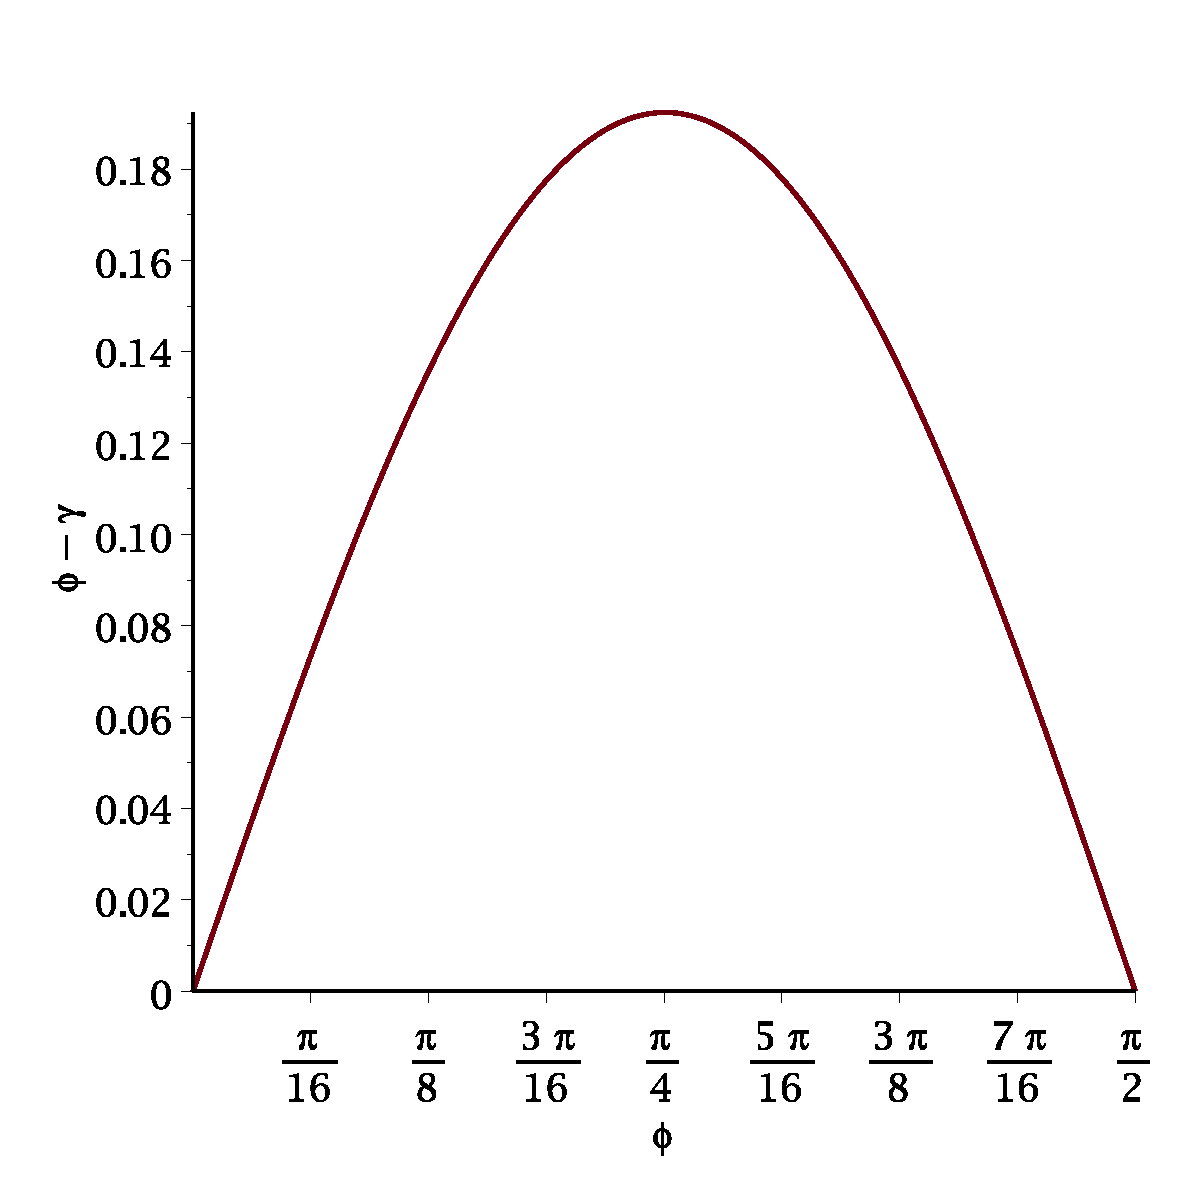
\includegraphics[width=3.25in,keepaspectratio]{wvs-146-4} \\
\end{floatingfigure}

From the figure on page \pageref{geometric-figure},
$\angle(\vec{P},\vec{G}) = \phi - \gamma = \cos^{-1} (\mathbf{g} \cdot
\hat{P})$.

Then (using Equations (\ref{tangents}))
%
\begin{equation}\begin{split}\label{phi-gamma}
\cos(\phi - \gamma) =\,& \cos \phi \cos \gamma + \sin \phi \sin \gamma =
\mathbf{g} \cdot \hat{P} \\
 = \,&
\frac{1-e^2 \sin^2 \phi}{\sqrt{\cos^2\phi + (1-e^2)^2 \sin^2\phi}}
\text{ and} \\
\tan(\phi - \gamma) =\,& \frac{e^2 \sin\phi \cos\phi}
                              {1-e^2 \sin^2 \phi}
                    = \frac{e^2 \sin\gamma \cos \gamma}
                           {1 - e^2 \cos^2 \gamma } \\
                    =\,& \frac{e^2 \sin\theta \cos \theta}{\sqrt{1-e^2}}
                    = \frac{e^2\, \sin 2 \theta}{2\sqrt{1-e^2}} \,,\\
\end{split}\end{equation}

which is obviously maximum for $\theta = \frac\pi4$.

From Equation (\ref{in-the-plane}), the angle $\phi-\gamma$ between the
gradient and geocentric position vectors is the angle between a profile
that is normal to the Earth surface (i.e., along a line of constant
longitude and geodetic latitude), and one that is along a line of constant
geocentric latitude.

Using $e^2 = 6.69437999014\!\times\!10^{-3}$ from WGS84 Table 3.3, the
largest value of $\phi-\gamma$ is 0\degs19242430116 at $\phi$ =
45\degs0962121506, $\gamma$ = 44\degs9037878494, $\theta = \frac\pi4$ =
45$^\circ$.  At that latitude and an altitude of 100 kilometers, the
distance between points on the two profiles is 335.843603774 meters.
% 
% \begin{minipage}[t]{0.48\textwidth}
% \begin{centering}
% Value of $\phi-\gamma$, degrees\\[14pt]
% 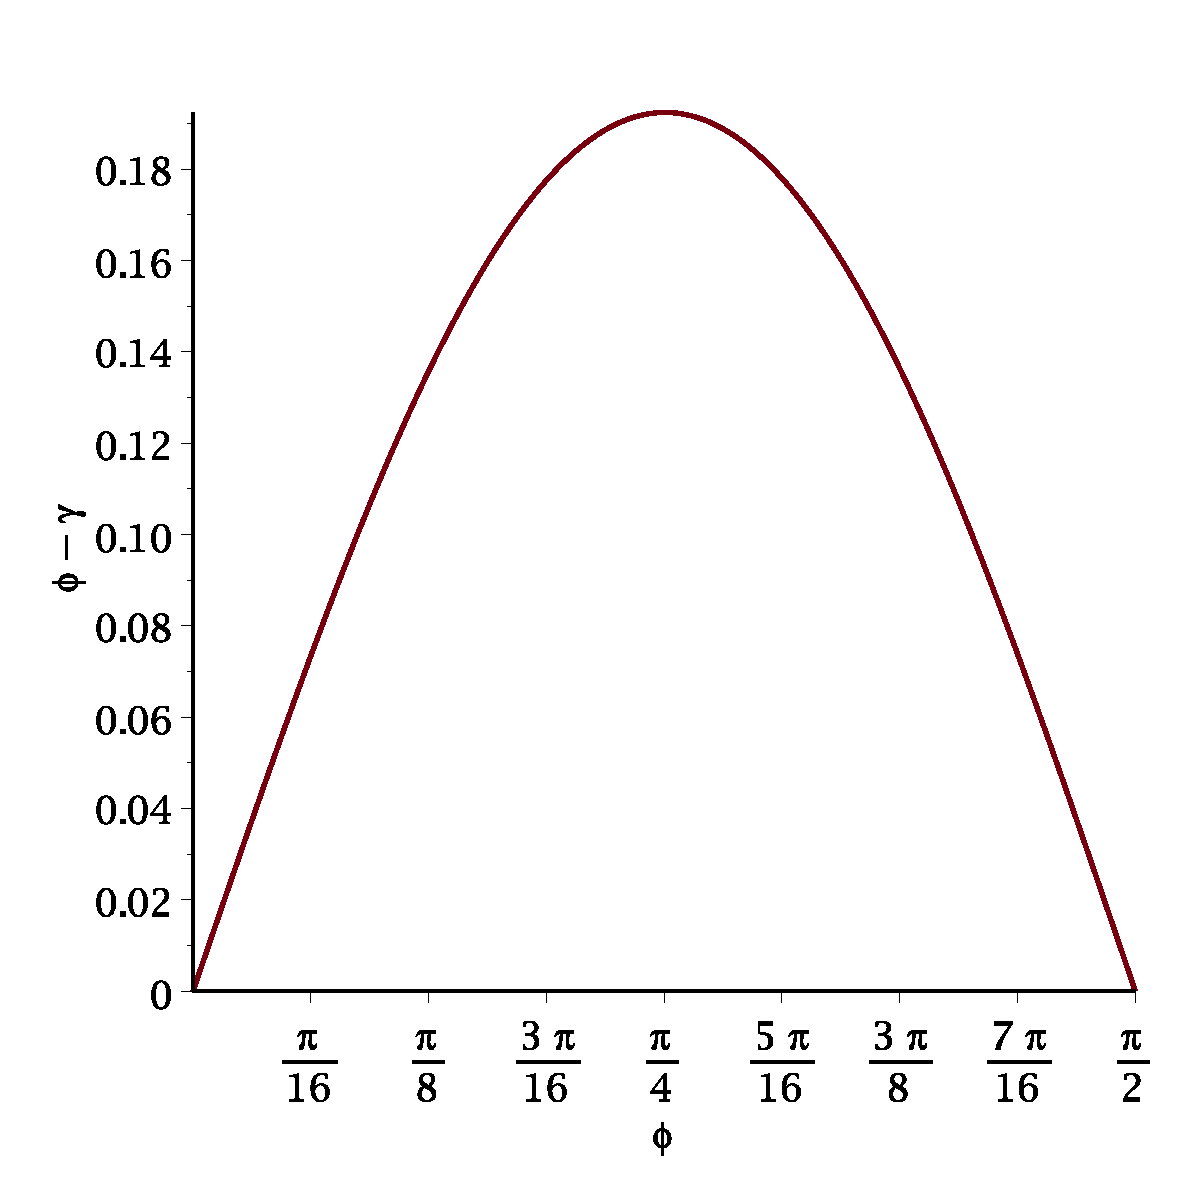
\includegraphics[width=0.98\textwidth,keepaspectratio]{wvs-146-4} \\
% \end{centering}
% \end{minipage}
% \begin{minipage}[t]{0.48\textwidth}
% \begin{centering}
% Distance $d$ of normal section\\
% from the center of the Earth\\[4pt]
% \includegraphics[width=0.98\textwidth,keepaspectratio]{wvs-146-5} \\
% \end{centering}
% \end{minipage}

%=========================================================================
\section{Relationship between 2-D and 3-D gradient vectors}

The angle between the gradient to the Earth surface and the gradient to
the orbit-plane projected ellipse, at the same point, is invariant with
respect to rotation about the $z$ (polar) axis.  Therefore, without loss
of generality, assume the orbit plane is rotated about the $x$ axis.

Let the Cartesian co\"ordinates of a point on the orbit plane be
$(\xi,\eta)$, where the $\xi$ axis is parallel to the $x$ axis and the
$\eta$ axis is orthogonal to the $\xi$ axis.  Then the three-dimensional
co\"ordinates of that point are

\begin{equation}\label{xyz}
\left[ \begin{array}{l} x \\ y \\ z  \end{array} \right] = 
\left[ \begin{array}{l} \xi \\ \eta\cos\beta \\ \eta \sin\beta
 \end{array} \right] \,,
\end{equation}

where $\beta$ is the angle of inclination. The equation of the orbit-plane
projected ellipse can be written

\begin{equation}\label{orbit-plane-ellipse}
\Sigma_p = \xi^2 + \frac{\eta^2}{1 - \epsilon^2} = a^2 \,,
\text{ and its gradient } \nabla\Sigma_p = \vec{G}_p =
2 \xi + \frac{2 \eta}{1-\epsilon^2},
\end{equation}

where

\begin{equation}\label{epsilon2}
\epsilon^2 = 1 - \frac{b^2}{a^2}
           = \frac{e^2 \sin^2\beta}{1-e^2 \cos^2 \beta}
\text{ and }
1 - \epsilon^2 = \frac{1-e^2}{1-e^2\cos^2\beta}\,,
\end{equation}

\newcommand{\OP}{p}

and $b$ is given by Equation (\ref{b2}).  Let $\OP$ be the geodetic angle
within the orbit plane to $\Sigma_p$.  Then the parametric equations for
$\Sigma_p$, analogously to Equations (\ref{nine}), are

\begin{equation}\begin{split}
\xi =  \,& \frac{a\, \cos\OP}{\sqrt{1-\epsilon^2\cos^2\OP}} \\
\eta = \,& \frac{a\, (1-\epsilon^2)\sin\OP}
                {\sqrt{1-\epsilon^2\cos^2\OP}} \,, \\
\end{split}\end{equation}

and the unit gradient within the orbit plane, analogously to the
definition of the unit gradient $\mathbf{g}$ to the Earth surface in
Equation (\ref{unit-gradient}), is
%
\begin{equation}
\frac{\vec{G}_p}{| \vec{G}_p |} =
\mathbf{g}_p =
\left[ \begin{array}{l} \cos\OP \\ \sin\OP \\ \end{array} \right]
\text{; its three-dimensional components are }
\left[ \begin{array}{l} \cos\OP \\
                        \sin\OP\cos\beta \\
                        \sin\OP\sin\beta \\ \end{array} \right] \,.
\end{equation}

Then the angle $\Gamma$ between the gradients is given by
%
\begin{equation}\label{cosG}
\cos\Gamma =
\mathbf{g} \cdot \mathbf{g}_p =
\cos\phi ( \cos\lambda \cos\OP +
           \sin\lambda \sin\OP\, \cos\beta ) +
\sin\phi \sin\OP \, \sin\beta \,.
\end{equation}

To reduce this to a relationship involving only $\OP$ and $\beta$, use
Equations (\ref{nine}) to compute
%
\begin{equation}\begin{split}\label{lambdaphi}
\tan\lambda = \,& \frac{y}x \\
\tan\phi = \,& \frac{z}{(1-e^2)\rho} = \frac{z}{(1-e^2)\sqrt{x^2+y^2}}
\,.
\end{split}\end{equation}
%
Using Equations (\ref{xyz}) and
%
\begin{equation}\begin{split}\label{aux}
G = \,& 1-e^2,\, W=1-G^2 = e^2(2-e^2),\, H = 1-e^2\cos^2\beta,\,
        E = 1 - \epsilon^2 = \frac{G}H \,, \\
S^2 = \,& E^2 \cos^2\beta\,\sin^2\OP + \cos^2\OP
    = \frac{G^2}{H^2} \cos^2\beta\,\sin^2\OP + \cos^2\OP\, \text{, and} \\
T   = \,& S^2\,H^2 + \sin^2\beta\,\sin^2\OP
    = (1-W\cos^2\beta)(1-W\cos^2\beta\,\cos^2\OP)
\\
    = \,& (1-e^2(2-e^2)\cos^2\beta)(1-e^2(2-e^2)\cos^2\beta\,\cos^2\OP)
    \,, \\
\end{split}\end{equation}
Equations (\ref{lambdaphi}) become
\begin{equation}\begin{split}\label{lambda-phi-def}
\tan\lambda = \,& \frac{\eta\cos\beta}{\xi}
            = E \cos\beta\, \tan\OP
            = \frac{G \cos\beta\, \tan\OP}H \\
\cos\lambda = \,& \frac{\cos\OP}S \\
\sin\lambda = \,& \frac{\sqrt{S^2-\cos^2\OP}}S
            = \frac{E \cos\beta\, \sin\OP}S
            = \frac{G \, \cos\beta\, \sin\OP}{SH} \\
\tan\phi = \,& \frac{\eta\sin\beta}
                {G\sqrt{\xi^2 + \eta^2\cos^2\beta}}
         = \frac{\sin\beta\,\sin\OP}{SH} \\
\cos\phi = \,& \frac{S H}{\sqrt{T}} \\
\sin\phi = \,& \frac{\sin\beta\,\sin\OP}{\sqrt{T}}\,. \\
\end{split}\end{equation}
%
Substituting Equations(\ref{lambda-phi-def}) into Equation (\ref{cosG}),
we have
%
\begin{equation}\begin{split}
\cos\Gamma = \,& \frac{H}{\sqrt{T}} ,\,
\frac{\partial \cos\Gamma}{\partial \OP}
 = -\frac{H}{2 T^\frac32} \frac{\partial T}{\partial \OP} \,\text{, and }
\frac{\partial \cos\Gamma}{\partial \beta}
 = \frac1{2 T^\frac32}
 \left[ 2 T \frac{\partial H}{\partial \beta} -
        H \frac{\partial T}{\partial \beta} \right] \,.
 \\
\end{split}\end{equation}
%
From Equations (\ref{aux}) we have
\begin{equation}\begin{split}
\frac{\partial T}{\partial \OP}
 = \,& 2 W ( 1 - W \cos^2\beta ) \cos^2\beta \, \cos\OP\, \sin\OP
 = \frac{2WT\cos^2\beta \, \cos\OP\, \sin\OP}
        {1-W\cos^2\beta\,\cos^2\OP}\,,  \\
\frac{\partial T}{\partial \beta}
 = \,& 2\, W \cos\beta \,\sin\beta
       ( 1 + ( 1 - 2\, W \cos^2\beta ) \cos^2\OP)\,, \\
\frac{\partial H}{\partial \OP} = \,& 0 \,\text{, and }
\frac{\partial H}{\partial \beta}
 = 2 e^2 \cos\beta\,\sin\beta \,. \\
\end{split}\end{equation}
%
$\frac{\partial \cos\Gamma}{\partial \OP}=0$ for $\beta=\frac\pi2$, $p=0$,
and $p=\frac\pi2$.  For $\beta=0$, $\beta=\frac\pi2$, or $\OP=0$,
$\Gamma=0$.  For $\OP=\frac\pi2$, $T = 1 - W \cos^2\!\beta$ and
%
\begin{equation}\begin{split}\label{solution}
\,& \frac{\partial \cos\Gamma}{\partial \beta} =
\frac{\cos\beta\,\sin\beta\,(W+e^2\,(2-W\,\cos^2\!\beta))}{T^\frac32}
= 0 \text{ when }
\cos^2\!\beta = \frac2W - \frac1{e^2} = \frac1{2-e^2}\,,
 \\
\,&\text{giving } \cos\Gamma = \frac{2\sqrt{1-e^2}}{2-e^2} \text{ or }
\tan\Gamma = \frac{e^2}{2\sqrt{1-e^2}}\,
\text{, the same result as Equation (\ref{phi-gamma}).}
\end{split}\end{equation}
%
Using $e^2 = 6.69437999014\!\times\!10^{-3}$ from WGS84 Table 3.3,
$\beta_0 =$ 44\degs9037878494 $\approx \frac{\pi}{4.0086}$ radians and
$\left.\Gamma\right|_{\beta_0} = $0\degs19242430116.  At an altitude of
100 kilometers, the horizontal positions on the two gradients are
different by 200000 $\sin\left(\frac12\Gamma\right)$ = 335.843603774
meters, the same result as in Section \ref{Relationship}.

\newcommand*{\mydprime}{^{\prime\prime}\mkern-1.2mu}
\newcommand{\secs}{$\stackrel{\hspace*{-0.5pt}\mydprime}{\vspace*{-2pt}.}$}

\begin{minipage}[t]{0.42\textwidth} Angle $\Gamma$ in degrees between
$\mathbf{g}$ and $\mathbf{g}_p$ for EOS AURA, which is in an orbit plane
inclined at 98\degs14.  The maximum value of $\Gamma$ is
0\degs0537688556, and the maximum distance between points on the two
profiles at an altitude of 100 kilometers is 93.8443530812 meters.\\[3pt]
\begin{centering}
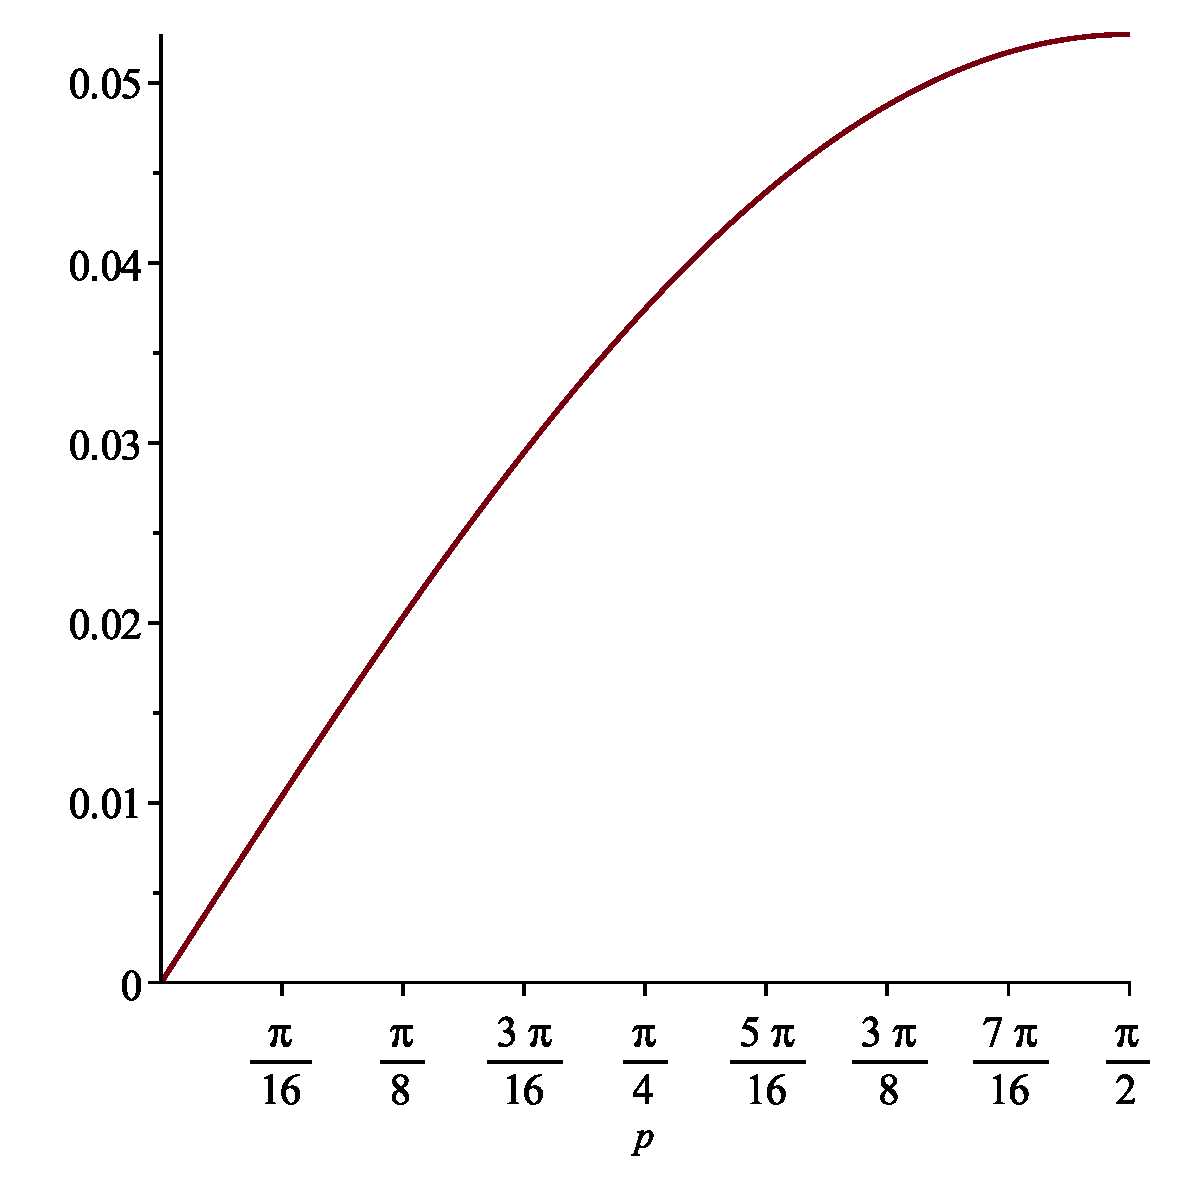
\includegraphics[width=0.95\textwidth,keepaspectratio]{wvs-146-6} \\
\end{centering}
\end{minipage}
%
\begin{minipage}[t]{0.55\textwidth}
\begin{centering}
Angle $\Gamma$ in degrees between $\mathbf{g}$ and $\mathbf{g}_p$ for\\
$0 \leq \OP \leq \frac\pi2$ and $0 \leq \beta \leq \frac\pi2$.\\[6pt]

\ifnum \pdfoutput>0 \vspace*{0.1in} \fi
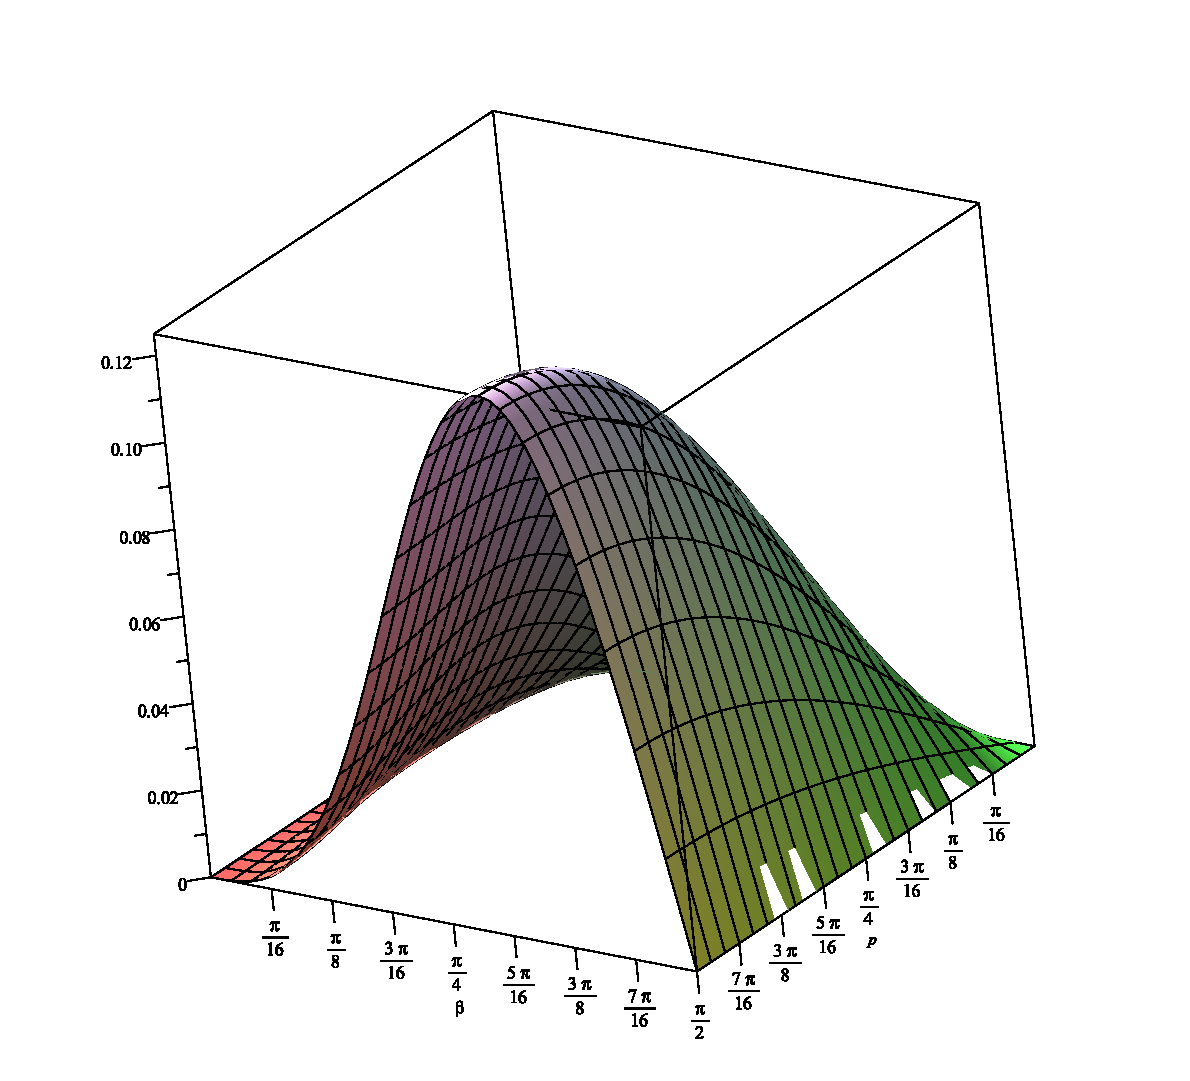
\includegraphics[width=1.2\textwidth,keepaspectratio,clip]{wvs-146-7} \\
%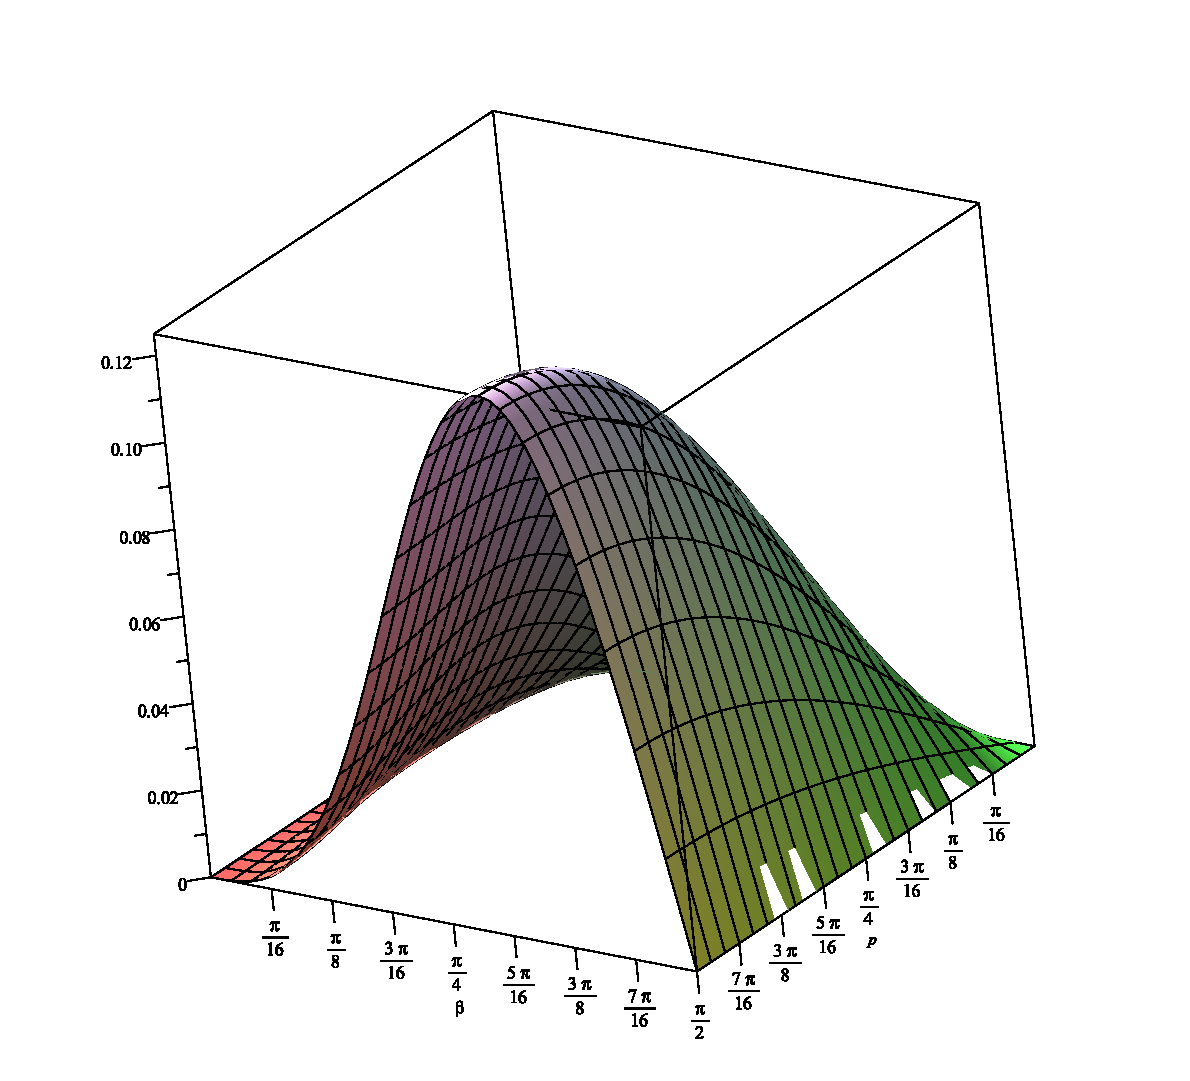
\includegraphics[scale=0.6]{wvs-146-7} \\
\end{centering}
\end{minipage}

\begin{minipage}[t]{0.5\textwidth}
Angle $\Gamma$ in degrees between $\mathbf{g}$ and $\mathbf{g}_p$ for
$p=\frac{\pi}2$.\\[3pt]
\begin{centering}
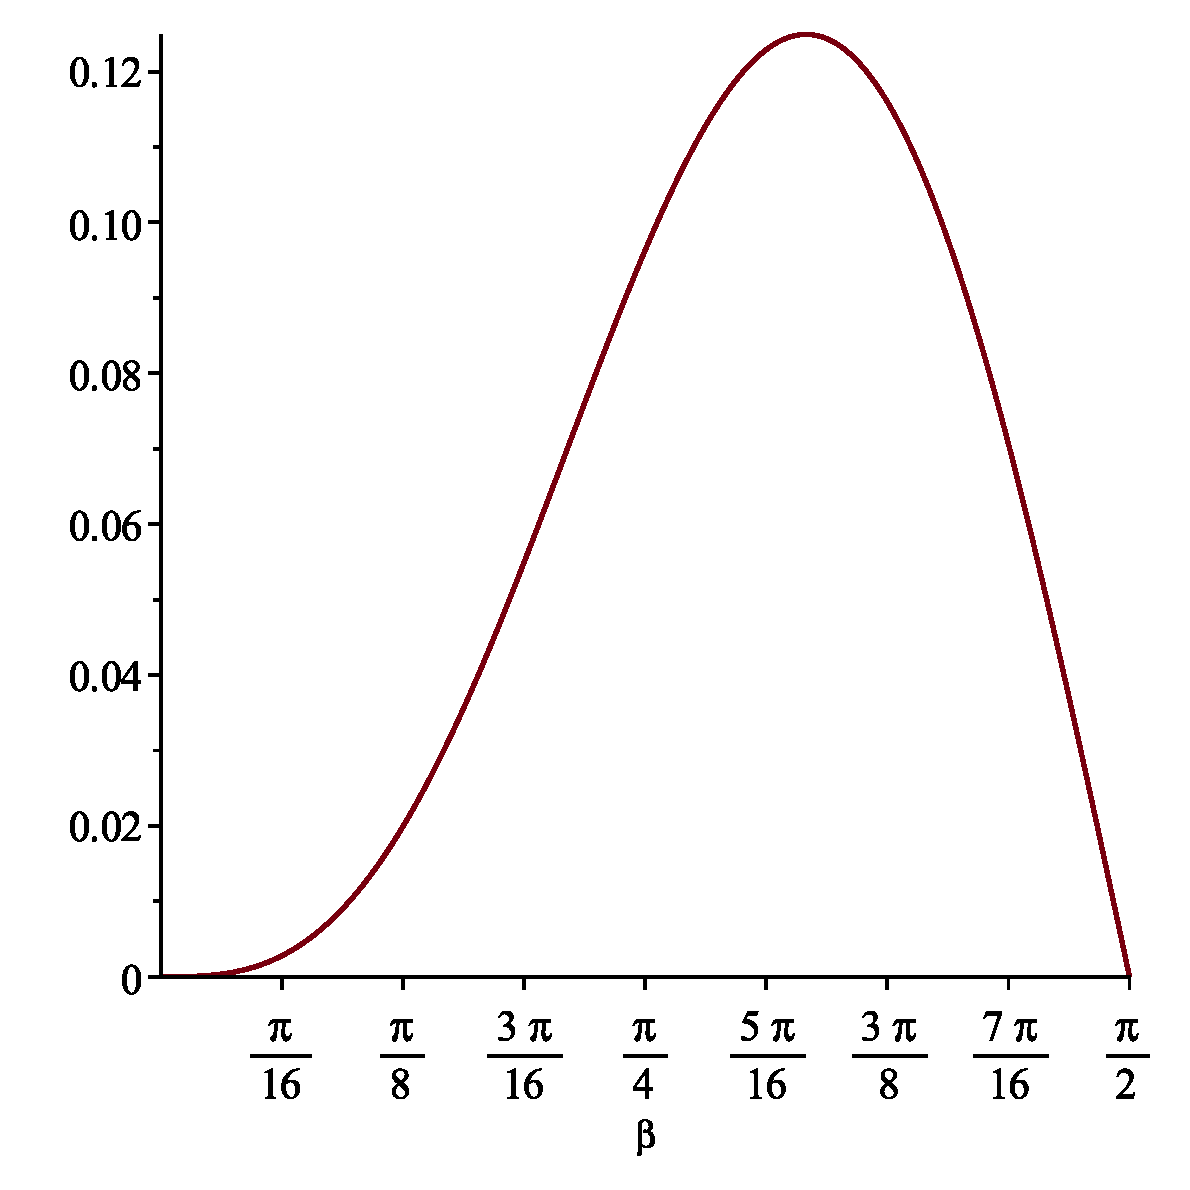
\includegraphics[width=0.95\textwidth,keepaspectratio]{wvs-146-8} \\
\end{centering}
\end{minipage}
\begin{minipage}[t]{0.45\textwidth}
Angle $\Gamma$ in degrees between $\mathbf{g}$ and $\mathbf{g}_p$ for
$\beta =$ 44\degs9037878494.\\[3pt]
\begin{centering}
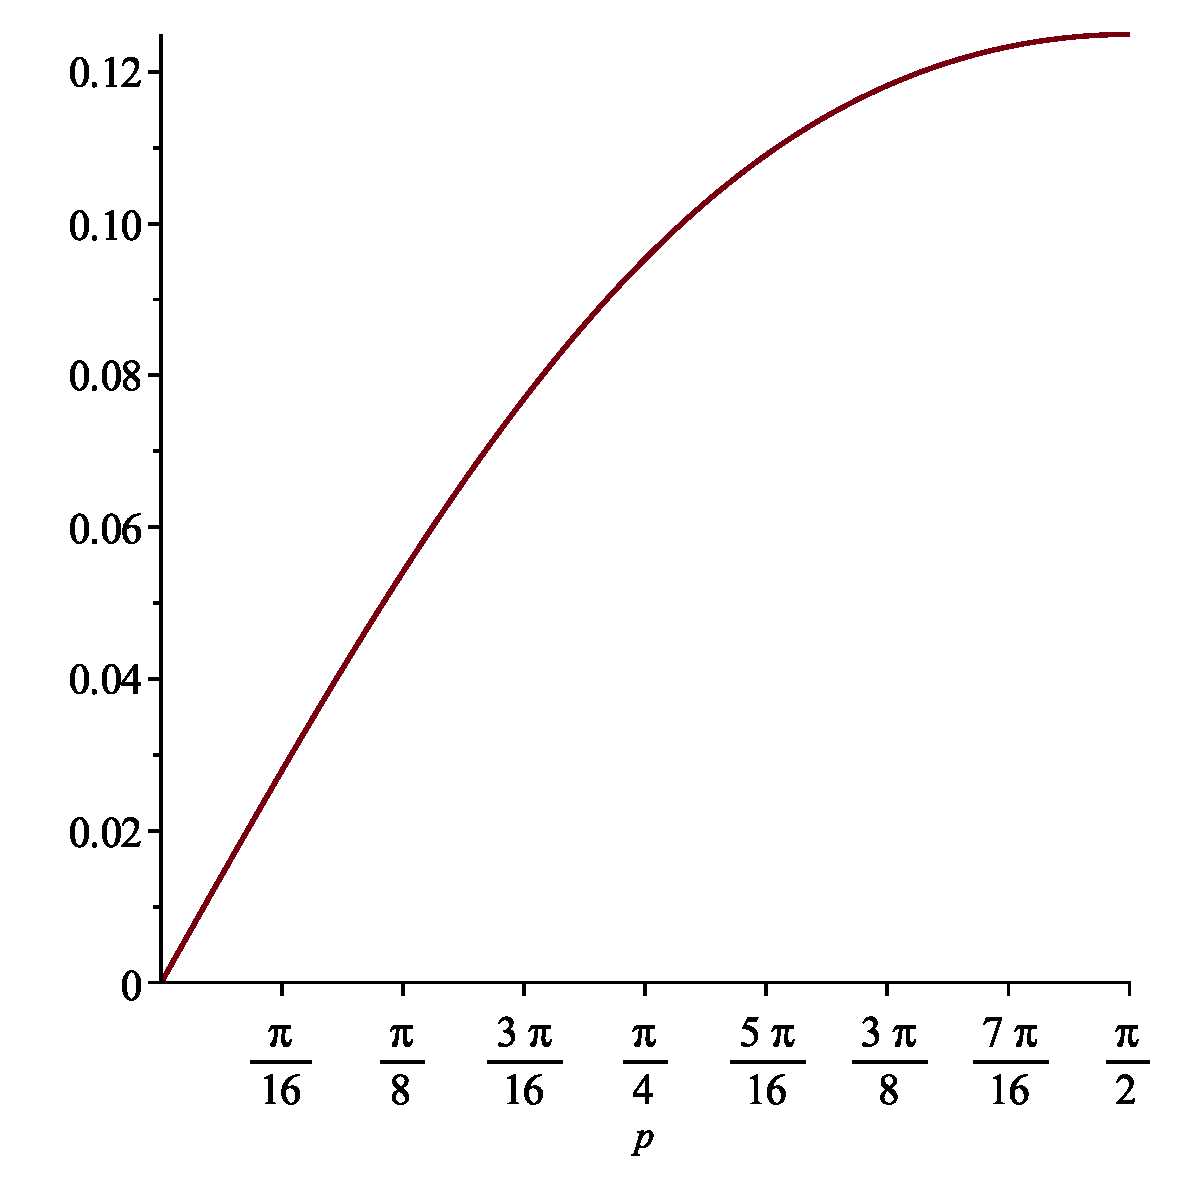
\includegraphics[width=0.95\textwidth,keepaspectratio]{wvs-146-9} \\
\end{centering}
\end{minipage}

\newpage
The projection of $\mathbf{g}$ into the orbit plane is parallel to
$\mathbf{g}_p$.  This can be verified by noting that

\begin{equation}\label{in-the-plane}
\mathbf{n}_p \cdot ( \mathbf{g} \times \mathbf{g}_p ) = 0\,\text{, where}
\end{equation}
%
\begin{equation}
\mathbf{n}_p = \left[ \begin{array}{c} 0 \\ -\sin\beta \\ \cos\beta
\end{array} \right]
\text{ is the normal to the plane and }
\frac{\mathbf{g} \times \mathbf{g}_p}
     {| \mathbf{g} \times \mathbf{g}_p |} =
\left[ \begin{array}{c}
 -\sin\OP \\ \cos\beta\cos\OP \\ \sin\beta\cos\OP \end{array} \right]\,.
\end{equation}

Therefore, $\Gamma = \sin^{-1} ( \mathbf{g} \cdot \mathbf{n}_p ) =
\sin^{-1} | \mathbf{g} \times \mathbf{g}_p |$.  For $p=\frac\pi2$,

\begin{equation}
| \mathbf{g} \times \mathbf{g}_p | =
 \frac{e^2 \cos\beta\sin\beta}{1-e^2\cos^2\beta} \text{ and }
\frac{\d | \mathbf{g} \times \mathbf{g}_p |}{\d \beta} =
-\frac{e^2(1-(2-e^2)\cos^2\beta)}{(1-e^2\cos^2\beta)^2} = 0 \text{ for }
\beta=\cos^{-1} \frac1{\sqrt{2-e^2}} \,,
\end{equation}

which is the same as Equations (\ref{phi-gamma}) and (\ref{solution}).

%=========================================================================
\newpage \section*{Appendix: Bowring's proof of prime vertical radius of
curvature} \label{appendix}

From \emph{Notes on the curvature in the prime vertical section}, {\bf
Survey Review 29}, 226 (October 1987) pp 195-196.

Let $P$ be a point on the reference ellipsoid and let $A$ and $B$ be two
points on the prime vertical section through $P$ such that $A$ and $B$ are
symmetrically placed about $P$ (see the figure below).  Let the normals to
the ellipsoid at $A$ and $B$ intersect at $G$ on the minor axis.  (This is
so because by symmetry about the meridian through $A$ the normal at $A$
intersects the minor axis, and similarly for the normal at $B$. 
Furthermore the points at $A$ and $B$ are at the same latitude and
therefore the normals intersect the minor axis at the same point).

Let the plane $ABG$ intersect the surface in the line $AP'B$.  Then AG is
perpendicular to the line $AP'B$ at $A$ (because $AG$ is perpendicular to
all surface lines through $A$), and similarly $BG$ is perpendicular to the
line at $B$.  Let now $A$ and $B$ approach $P$ (on the prime vertical
section) \emph{simultaneously} and \emph{symmetrically}.  Then $AP'B
\rightarrow APB$, and at all times the normals at the ends intersect on
the minor axis.  This is the geometrical evidence that the centre of
curvature lies on the minor axis, and therefore the centre of curvature
$C$ of the prime vertical section through $P$ lies on the intersection of
the normal at $P$ (to the ellipsoid) with the minor axis, and the radius
of curvature is equal to the length $CP$.

\begin{centering}
\includegraphics[scale=1.0]{wvs-146-2}\\
\end{centering}

\newpage \section*{Appendix: Curvatures for general ellipsoid}

%-------------------------------------------------------------------------
\subsection*{Using reduced latitude}

\begin{equation}
\mathbf{r} = \left[ \begin{array}{l}
a\, \cos\theta \cos\lambda \\
b\, \cos\theta \sin\lambda \\
c\, \sin\theta
\end{array} \right]
\end{equation}

\begin{equation}
\begin{array}{lll}
\frac{\partial \mathbf{r}}{\partial \lambda} =
\left[ \begin{array}{l}
-a\, \cos \theta \sin \lambda \\
b\, \cos \theta \cos \lambda \\
0
\end{array} \right] &
\frac{\partial \mathbf{r}}{\partial \theta} =
\left[ \begin{array}{l}
-a\, \sin \theta \cos \lambda \\
-b\, \sin \theta \sin \lambda \\
c\, \cos \theta \\
\end{array}
\right] & \\
 & & \\
\frac{\partial^2 \mathbf{r}}{\partial \lambda^2} =
\left[ \begin{array}{l}
-a\, \cos \theta \cos \lambda \\
-b\, \cos \theta  \sin \lambda\\
0
\end{array} \right] &
\frac{\partial^2 \mathbf{r}}{\partial \lambda\, \partial \theta} =
\left[ \begin{array}{l}
a\, \sin \theta \sin \lambda \\
-b\, \sin \theta \cos \lambda\\
0 \\[10pt]
\end{array} \right ] &
\frac{\partial^2 \mathbf{r}}{\partial \theta^2} =
\left[ \begin{array}{l}
-a\, \cos \theta \cos \lambda \\
-b\, \cos \theta \sin \lambda \\
-c\, \sin \theta
\end{array} \right] \\
\end{array}
\end{equation}

\begin{equation}\begin{split}
\mathbf{N} =\,& \frac{\partial \mathbf{r}}{\partial \lambda} \times
             \frac{\partial \mathbf{r}}{\partial \theta}\,
           =
           \left[ \begin{array}{l}
             b\, c\, \cos \lambda \cos^2 \theta \\
             a\, c\, \sin \lambda \cos^2 \theta \\
             a\,b\, \sin \theta \cos \theta
            \end{array} \right]
\\[3pt]
|\mathbf{N}|
 = \,& \cos\theta
     \sqrt{c^2 ( a^2 \sin^2\lambda + b^2 \cos^2\lambda ) \cos^2\theta
           + a^2 \, b^2 \sin^2\theta} ,\,
\mathbf{g} = \frac{\mathbf{N}}{|\mathbf{N}|} \\
\end{split}\end{equation}

\begin{equation}\begin{split}
E = \,& \frac{\partial \mathbf{r}}{\partial \lambda} \cdot
        \frac{\partial \mathbf{r}}{\partial \lambda}
  = ( a^2 \sin^2\lambda + b^2 \cos^2\lambda ) \cos^2\theta \\
F = \,& \frac{\partial \mathbf{r}}{\partial \lambda} \cdot
        \frac{\partial \mathbf{r}}{\partial \theta}
  =(a^2 - b^2 ) \sin\lambda \cos\lambda \sin\theta \cos\theta \\
G = \,& \frac{\partial \mathbf{r}}{\partial \theta} \cdot
        \frac{\partial \mathbf{r}}{\partial \theta}
  = ( a^2 \cos^2\lambda + b^2 \sin^2\lambda ) \sin^2\theta +
        c^2 \cos^2 \theta \\
\end{split}\end{equation}

\begin{equation}\begin{split}
e = \,& \mathbf{g} \cdot
        \frac{\partial^2 \mathbf{r}}{\partial \lambda^2}
  = \frac{a\,b\,c\,cos^3\theta}{|\mathbf{N}|} \,.\\
f = \,& \mathbf{g} \cdot
        \frac{\partial^2 \mathbf{r}}{\partial \lambda \partial \theta}
  = 0 \\
g = \,& \mathbf{g} \cdot
        \frac{\partial^2 \mathbf{r}}{\partial \theta^2}
  = \frac{a\, b \, c\,\cos\theta}{|\mathbf{N}|} \\
\end{split}\end{equation}

\begin{equation}\begin{split}
\kappa = \,& \frac{a b c \cos\theta}{2A}\, \left(
             \frac{(((a^2-b^2)\cos^2\lambda-c^2)\cos^2\theta
             -b^2 \sin^2\theta - a^2)}{|\mathbf{N}|}
             \pm |\mathbf{N}| \sqrt{W} \right) \text{, where} \\
A =\,& E G - F^2 = c^2 ( a^2 - ( a^2-b^2 ) \cos^2\lambda ) \cos^2\theta
                + a^2 b^2 \sin^2\theta \text{, and} \\
W =\,& (a^2\cos^2\lambda + b^2\sin^2\lambda -c^2 ) \cos^4\theta +
       2 ( a^2-b^2)(b^2\sin^2\lambda - ( a^2 - 2 c^2 ) \cos^2\lambda
         -c^2 ) \cos^2 \theta \\
   \,& + (a^2-b^2)^2 \,.
\end{split}\end{equation}

Gaussian curvature:
%
\begin{equation}
K = \kappa_1 \, \kappa_2
  = \left( \frac{a\, b\, c}
                {c^2 ( a^2 \sin^2\lambda + b^2 \cos^2\lambda )
                 \cos^2\theta + a^2 b^2 \sin^2\theta }
    \right)^2 \,.
\end{equation}

Radius of Gaussian curvature:

\begin{equation}
R = \frac{1}{\sqrt{K}} =
 \frac{c}{ab} \left( a^2 \sin^2\lambda
 + b^2 \cos^2\lambda \right) \cos^2\theta
 + \frac{ab}c \sin^2\theta \,.
\end{equation}

%-------------------------------------------------------------------------
\subsection*{Using geocentric latitude}

\begin{equation}\begin{split}
\mathbf{r} = \,&  R\, \vec{\rho} \text{ where }
  \vec{\rho} = \left[ \begin{array}{l}
  \cos\gamma \cos\lambda \\
  \cos\gamma \sin\lambda \\
  \sin\gamma
\end{array} \right] \text{ and} \\
R = \,& \frac{abc}
         {\sqrt{ c^2 ( b^2 \cos^2\lambda + a^2 \sin^2\lambda ) \cos^2\gamma
               + a^2 b^2 \sin^2\gamma}} \\
\end{split}\end{equation}

\begin{equation}\begin{split}
\frac{\partial R}{\partial \lambda} = \,& R_\lambda = R^3
 \left( \frac1{a^2}-\frac1{b^2} \right) \sin\lambda \cos\lambda \cos^2\eta \\
\frac{\partial R}{\partial \gamma} = \,& R_\gamma = R^3
 \left( \frac{\sin^2\lambda}{b^2} + \frac{\cos^2\lambda}{a^2}-\frac1{c^2}
  \right) \sin\eta \cos\eta \\
\frac{\partial^2 R}{\partial \lambda \partial \gamma} = \,& R_{\lambda\gamma}
= R^5 \left( \frac1{a^2} -\frac1{b^2} \right)
  \sin\gamma\cos\gamma \sin\lambda\cos\lambda
  \left( \left( \frac{\sin^2\lambda}{b^2} +\frac{\cos^2\lambda}{a^2}
                -\frac3{c^2} \right) + 2\,\frac{\sin^2\gamma}{c^2}
  \right)
\end{split}\end{equation}

\begin{equation}\begin{array}{ll}
\frac{\partial \vec{\rho}}{\partial \lambda} = \vec{\rho}_{\lambda} =
\cos\gamma
\left[ \begin{array}{l} -\sin\lambda \\
                         \cos\lambda \\
                          0 \end{array} \right] &
%
\frac{\partial \vec{\rho}}{\partial \gamma} = \vec{\rho}_{\gamma} =
\left[ \begin{array}{l} -\sin\gamma \cos\lambda \\
                          -\sin\gamma \sin\lambda \\
                          \cos\gamma \end{array} \right] \\
%
\frac{\partial \mathbf{r}}{\partial \lambda} = \mathbf{r}_{\lambda} =
R\, \vec{\rho}_{\lambda} + \vec{\rho}\, R_{\lambda} &
%
\frac{\partial \mathbf{r}}{\partial \gamma} = \mathbf{r}_{\gamma} =
R\, \vec{\rho}_{\gamma} + \vec{\rho}\, R_{\gamma}
\end{array}\end{equation}

\begin{equation}\begin{array}{ll}
\mathbf{N} = R \left(
 \cos\gamma\,  ( \mathbf{r} - R_\gamma \rho_{\gamma} )
 - R_\lambda \, \frac{\rho_{\lambda}}{\cos \gamma}
 \right) &
\mathbf{|N|} = R
 \sqrt{ \left( R^2 + R_\gamma^2
        \right) \cos^2\gamma
      + R_\lambda^2} \\
\mathbf{g} = \frac{\mathbf{N}}{\mathbf{|N|}}
\end{array}\end{equation}

\begin{equation}\begin{array}{ll}
\frac{\partial^2 \vec{\rho}}{\partial \lambda^2}
 = \vec{\rho}_{\lambda\lambda} = -\cos\gamma
  \left[ \begin{array}{l} \cos\lambda \\ \sin\lambda \\ 0
  \end{array} \right] &
\frac{\partial^2 \vec{\rho}}{\partial \lambda \partial\gamma}
 = \vec{\rho}_{\lambda\gamma} = -\sin\gamma
  \left[ \begin{array}{l} \sin\lambda \\ \cos\lambda \\ 0
  \end{array} \right] \\[3pt]
\frac{\partial^2 \vec{\rho}}{\partial \gamma^2}
 = \vec{\rho}_{\gamma\gamma} =
  -\left[ \begin{array}{l} \cos\gamma\cos\lambda \\ \cos\gamma\sin\lambda \\
   \sin\eta
  \end{array} \right] \\
\end{array}\end{equation}
%
\begin{equation}\begin{array}{ll}
\frac{\partial^2 \mathbf{r}}{\partial \lambda^2}
 = \mathbf{r}_{\lambda\lambda} =
 R \rho_{\lambda\lambda} + R_{\lambda} \rho_{\lambda}
 + \rho R_{\lambda\lambda} &
\frac{\partial^2 \mathbf{r}}{\partial \lambda \partial\gamma}
 = \mathbf{r}_{\lambda\gamma} =
 R \rho_{\lambda\gamma} + R_{\gamma} \rho_{\lambda}
 + \rho R_{\lambda\gamma} \\
\frac{\partial^2 \mathbf{r}}{\partial \gamma^2}
 = \mathbf{r}_{\gamma\gamma} =
 R \rho_{\gamma\gamma} + R_{\gamma} \rho_{\gamma}
 + \rho R_{\gamma\gamma} &
\end{array}\end{equation}

\begin{equation}\begin{array}{ll}
\frac{\partial \mathbf{r}}{\partial \lambda} = \mathbf{r}_{\lambda} =
R\, \vec{\rho}_{\lambda} + \vec{\rho}\, R_{\lambda} &
%
\frac{\partial \mathbf{r}}{\partial \gamma} = \mathbf{r}_{\gamma} =
R\, \vec{\rho}_{\gamma} + \vec{\rho}\, R_{\gamma}
\end{array}\end{equation}
%
\begin{equation}\begin{array}{lll}
E = \frac{\partial \mathbf{r}}{\partial \lambda} \cdot
    \frac{\partial \mathbf{r}}{\partial \lambda} 
  =  R^2 \cos^2\eta + R_\lambda^2 &
F = \frac{\partial \mathbf{r}}{\partial \lambda} \cdot
    \frac{\partial \mathbf{r}}{\partial \gamma} 
  = R_\lambda \, R_\gamma &
G = \frac{\partial \mathbf{r}}{\partial \gamma} \cdot
    \frac{\partial \mathbf{r}}{\partial \gamma}
  = R^2 + R_\gamma^2
\end{array}\end{equation}
%
\begin{equation}\begin{split}
e =\,& -\frac{ \cos\gamma ( \sin\gamma \cos\gamma R_\gamma R
             + \cos^2\gamma\, R^2 + 2 R_\lambda^2
             - R\, R_{\lambda\lambda}}{|\mathbf{N}|} \\
f =\,& \frac{ (R\,R_{\lambda\gamma} - R_\gamma\,R_\lambda) \cos\eta
            + R\, R_\lambda \, \sin\gamma}{|\mathbf{N}|} \\
g =\,& \cos\eta\,\frac{R\,( R_{\gamma\gamma} - R) - 2 R_\gamma^2}
                      {|\mathbf{N}|}
\end{split}\end{equation}

\begin{equation}\label{kappa-gen}
\kappa = \frac{(e G + g E - 2 f F ) \pm
               \sqrt{ (e G + g E - 2 f F )^2 - 4 ( E G - F^2) ( e g - f^2)}}
              { 2 ( E G - F^2) }
\end{equation}

Even without expanding $E$, $F$, $G$, $e$, $f$, and $g$, the roots
$\kappa$ of Equation (\ref{third}), the values of Equation
(\ref{kappa-gen}), each occupy four lines. Expanding completely, they
occupy 60 lines.

%-------------------------------------------------------------------------
\subsection*{Using geodetic latitude}

Geodetic latitude is not well defined for a general ellipsoid -- it
depends upon longitude.

\label{lastpage}
\vspace*{-0.1in} % Somehow, this causes lastpage to be defined
\end{document}

\newpage
\begin{equation}\begin{split}
G = \,& \, 1-e^2 \\
%
H = \,& 1 -e^2 \cos^2\beta \\
%
\frac{\d H}{\d\beta} = \,& 2\,e^2 \cos\beta\,\sin\beta \\
%
\epsilon^2 = \,& \frac{e^2 \sin^2\beta}{1-e^2\cos^2\beta} =
             \frac{(1-G)\sin^2\beta}H;\,
             1-\epsilon^2 = \frac{G}H \\
%
\xi = \,& \frac{\cos\OP}{\sqrt{1-\epsilon^2\cos^2\OP}} =
      \frac{\sqrt{H} \, \cos\OP}{\sqrt{H-e^2\cos^2\OP\,\sin^2\beta}} \\
%
\eta = \,& \frac{G \sqrt{H}\sin\OP}
                {\sqrt{H - e^2\cos^2\OP\,\sin^2\beta )}} = G\, \xi \tan\OP \\
%
\tan\lambda = \,& \frac{y}x = \frac{\eta \cos\beta}{\xi} =
              \frac{G \sin\OP\, \cos\beta}{\cos\OP} =
              G \cos\beta\, \tan\OP \\
%
S^2 = \,& G^2 \sin^2\OP\, \cos^2\beta + \cos^2\OP \\
%
\frac{\partial S}{\partial \OP} = \,&
-\frac{(1-G^2\cos^2\beta)\cos\OP\sin\OP}S \\
%
\frac{\partial S}{\partial\beta} = \,&
 \frac{G^2 \sin^2\OP\, \cos\beta\sin\beta}S \\
%
\sin\lambda = \,& \frac{G \sin\OP\,\cos\beta}S \\
%
\cos\lambda = \,& \frac{\cos\OP}S \\
%
\tan\phi = \,& \frac{z}{G \rho} = \frac{Z}{G\sqrt{x^2+y^2}} =
           \frac{\eta\sin\beta}{G\sqrt{\xi^2+\eta^2\cos^2\beta}} =
           \frac{\sin\OP\sin\beta}S \\
%
T^2 = \,& S^2 + \sin^2\OP\, \sin^2\beta =
          1 - (1-G^2) \cos^2\beta\,\sin^2\OP \\
%
\frac{\partial T}{\partial \OP} = \,&
 \frac{\sin\OP\cos\OP\sin^2\beta + S\,\frac{\partial S}{\partial \OP}}T =
 \frac{(1-G^2) \cos^2\beta\,\cos\OP\sin\OP}T\\
%
\frac{\partial T}{\partial\beta} = \,&
 \frac{\sin^2\OP\,\cos\beta\sin\beta +
       S\, \frac{\partial S}{\partial\beta}}T =
 \frac{(1-G^2)\cos\beta\,\sin\beta\,\sin^2\OP}T
 \\
%
\sin\phi = \,& \frac{\sin\OP\sin\beta}T \\
%
\cos\phi = \,& \frac{S}T \\
%
\cos\Gamma = \,& \frac{1-e^2\cos^2\beta\,\sin^2\OP}T =
                 \frac{1-e^2\cos^2\beta\,\sin^2\OP}
                      {\sqrt{1 - (1-G^2) \cos^2\beta\,\sin^2\OP}} \\
%
\frac{\partial \cos\Gamma}{\partial \OP} = \,&
        -\frac{2 e^2 \cos^2\beta\,\cos\OP\sin\OP}T -
        \frac{1-e^2\cos^2\beta\,\sin^2\OP}{T^2} \,
        \frac{\partial T}{\partial \OP} =
     2 \cot\OP \left( \cos\Gamma-\frac1T\right) -
      \frac{\cos\Gamma}T\, \frac{\partial T}{\partial \OP} \\
%
\frac{\partial \cos\Gamma}{\partial \beta} = \,&
  \frac{2 \, e^2 \cos\beta \sin\beta\,\sin^2\OP}T -
   \frac{1-e^2\cos^2\beta\,\sin^2\OP}{T^2}
   \frac{\partial T}{\partial \beta} =
  -2\tan\beta \left(\cos\Gamma-\frac1T\right) -
   \frac{\cos\Gamma}T\, \frac{\partial T}{\partial \beta} \\
%
\end{split}\end{equation}

\begin{equation}\begin{split}
\frac{\partial \cos\Gamma}{\partial \OP} = \,&
\frac{\partial \cos\Gamma}{\partial \beta} = 0 \text{ when }
\sin\OP = \frac1{\sqrt{2-e^2}\cos\beta} \text{, for which} \\
\cos\Gamma =\,& \frac{2\sqrt{1-e^2}}{2-e^2} \\
\end{split}\end{equation}

Using $e^2 = 6.69437999014\!\times\!10^{-3}$ from WGS84 Table 3.3,
$\beta_0 =$ 44\degs9037878558 $\approx \frac{\pi}{4.0086}$ radians and
$\left.\Gamma\right|_{\beta_0} = $0\degs192424295874.  At an altitude of
100 kilometers, the horizontal positions on the two gradients are
different by 200000 $\sin(\frac12\Gamma)$ = 335.843594550 meters.

% $Id$

% $Log$
% Revision 1.14  2020/04/07 22:59:24  vsnyder
% Clarifications, correct some typos, add material about general ellipsoid.
%
% Revision 1.13  2020/03/28 04:09:44  vsnyder
% Add labels for other documents to reference
%
% Revision 1.12  2020/03/23 19:19:46  vsnyder
% Collect material about differential geometry in one section. Add derivation
% of angle between gradient to surface and gradient to orbit plane. Other
% improvements and corrections.
%
% Revision 1.11  2020/03/05 02:10:26  vsnyder
% Correct some typos, more details of dGamma/dBeta solution
%
% Revision 1.10  2020/03/03 02:27:38  vsnyder
% Correct typos before Equation (84) and in Equation (85)
%
% Revision 1.9  2020/03/03 01:41:24  vsnyder
% I think it's finally correct
%
% Revision 1.8  2020/02/13 02:49:04  vsnyder
% Repair a typo
%
% Revision 1.7  2020/02/13 02:06:29  vsnyder
% Significant update.  Added 2D-vs-3D gradient angle calculation
%
% Revision 1.5  2020/01/08 21:35:22  vsnyder
% Add labels for reference in wvs-157
%
% Revision 1.4  2020/01/06 21:20:17  vsnyder
% Substantial revision and additions
%
% Revision 1.3  2019/11/13 01:33:03  vsnyder
% Added a lot more material
%
% Revision 1.2  2017/10/13 19:10:51  vsnyder
% Add CVS stuff
%
